\documentclass[a4paper,12pt]{tesiinfo}
%\documentclass[a4paper,12pt,dvipdfm]{tesiinfo}

\usepackage{amsfonts}
\usepackage{amsmath}
\usepackage{latexsym}
\usepackage{tabularx}
\usepackage[english]{babel}
\usepackage[bookmarks=true]{hyperref}
\usepackage{subfigure}
\usepackage{graphicx}
\usepackage{amssymb}

%FROM UNI - NOT INCLUDED IN BASIC COMMANDS
\usepackage{fncychap}

%ADDS SYMBOLS FOR MATH OPERATIONS: CEIL and FLOOR
\usepackage{mathtools}
\DeclarePairedDelimiter\ceil{\lceil}{\rceil}
\DeclarePairedDelimiter\floor{\lfloor}{\rfloor}

%EQUISPACES THE FRACTIONS
\usepackage{multicol}
\usepackage{fixmath}
\newcommand\ddfrac[2]{\frac{\displaystyle #1}{\displaystyle #2}}

%DISPLAY IMAGES CORRECTLY
\usepackage[export]{adjustbox}
\graphicspath{ {Images/} }
\usepackage{float}

%FOOTNOTES - FONT SIZE DECREASED
%\usepackage{lmodern}

%9pt \`e la dimensione del font footnote
%11pt \`e la spaziatura. Se impostato a <9pt=troppo piccolo, se >12pt= troppo grande
\renewcommand{\footnotesize}{\fontsize{9pt}{11pt}\selectfont}

%Imposta 9 simboli diversi per creare le note. Cos\`i evitiamo di confondere``le note" con``la notazione usata"
%1 - *
%2 - †
%3 - ‡
%4 - 
%5 - 
%6 - 
%7 - 
%8 - 
%9 - 
\renewcommand{\thefootnote}{\fnsymbol{footnote}}

%BOH
\hypersetup{final}


\titolo{Crittografia Ellittica}
\laureando{Marco Carolla}
\relatore{Gabriele Di Stefano}
\annoaccademico{2016-2017}

\begin{document}

\maketitle
\contentspage
\chapter{Introduzione}
Con la parola composta da ``\textit{scritto}" e ``\textit{grafia}" intendiamo quella tematica della sicurezza in generale che prende spunto dalla crittografia, una scrittura segreta, tale che non possa essere letta senza conoscere l'artificio usato nella corrispondenza. Parliamo di scrittura cifrata quando il risultato della lettura di un testo \`e anch'esso privo di significato apparente. La cifratura di un testo pu\`o essere fatta per:
\begin{itemize}
    \item ``\textit{trasposizione}" mediante la quale la traduzione del linguaggio chiaro in linguaggio segreto ha luogo con spostamento o inversione degli elementi chiari;
    \item ``\textit{sostituzione}" degli elementi del linguaggio con segni convenzionali che pur potendo essere di qualsiasi genere, sono in pratica quelli della normale scrittura, lettere o cifre, e ci\`o per consentire la trasmissione telegraficamente;
    \item ``\textit{sistema misto}" che combina le precedenti interponendole una dopo l'altra.
\end{itemize} 
La sostituzione letterale pu\`o essere monoalfabetica e polialfabetica secondo che ha luogo in base a uno o pi\`u alfabeti cifranti da adoperare contemporaneamente.
\\
\\
Sistemi di scrittura segreta furono adoperati gi\`a nel Medioevo  dove larga diffusione ebbe il \textit{sistema bizantino a trasposizione} e adoperato oltre che nei documenti anche nei manoscritti greci e adottato in alcune cancellerie regie occidentali, come in quella di Napoli (14$^\circ$ secolo). Il sistema  a sostituzione  fu amplissimo nelle cancellerie signorili del 15$^\circ$ e 16$^\circ$ secolo in cui venivano alternati numeri e segni arbitrari di origine cabalistica. Nel 16$^\circ$ secolo vi fu una vasta opera di sistemazione teorica della crittografia culminata nella elaborazione di pi\`u complessi sistemi miste che rappresentavano la sintesi di quelli adoperati sino ad allora. 
Svetonio narra come Cesare usasse nelle sue comunicazioni militari un sistema di cifra che consisteva nel sostituire ciascuna lettera con quella che la segue di un numero fisso di posizioni nell'alfabeto (cifrario di Cesare). Un sistema di questo tipo si dice monoalfabetico, in quanto ciascun simbolo del testo in chiaro \`e sostituito da un unico simbolo dell'alfabeto di cifra. Oggi non \`e pi\`u utilizzato perch\`e estremamente semplice da risolvere.
\\
La diffusione delle tecniche crittografiche nelle corti rinascimentali diede impulso alla generazione, nel periodo dal 1400 al 1700, di voluminosi codici nomenclatori, soprattutto per la corrispondenza diplomatica, e fece perfezionare le tecniche di cifratura, soprattutto per le comunicazioni militari.  Per la sostituzione polialfabetica si ricorse  all'uso di specifici apparecchi (crittografi) che consentissero di eseguire velocemente le difficoltose operazioni. L.B. Alberti costru\`i un dispositivo, costituito da due corone circolari mobili concentriche con incise  le lettere dell'alfabeto da far corrispondere tra i suoi dischi, per permettere una pi\`u rapida cifratura monoalfabetica ma, nel descriverne le modalit\`a d'uso, raccomandava che il crittografo, dopo aver scritto qualche parola, alterasse la posizione relativa dei due dischi, in modo da ottenere che simboli eguali venissero cifrati in maniera differente: \`e il principio della cifratura polialfabetica.
Un semplice metodo di cifratura polialfabetica, proposto da B. de Vigen\`ere nel 16$^\circ$ sec. e in uso ancora oggi, consiste nell'utilizzare alcune (o tutte) delle 26 possibili cifre di Cesare, sia progressivamente, sia in ordine arbitrario; la chiave di questo sistema consiste in una sequenza di caratteri, da riutilizzarsi ciclicamente per tutta la lunghezza del messaggio, che indica quale alfabeto \`e utilizzato per ciascuna lettera del testo in chiaro. La fortuna di questo metodo dipende dalla sua semplicit\`a, dalla sua variabilit\`a e dalla sua sicurezza. Nelle applicazioni militari, comunque, le difficolt\`a logistiche, nella distribuzione e variazione delle chiavi, ne limitano la lunghezza e ne rendono obbligatorio il riuso e, pertanto, anche i sistemi polialfabetici non possono considerarsi sicuri.
\\
Un sistema proposto, verso la fine del 19$^\circ$ sec., da  C. Wheatstone e adottato nella Seconda guerra mondiale, consiste nel disporre i simboli dell'alfabeto secondo un quadrato di  Polibio e rappresentare coppie di caratteri con le seguenti regole: a) se entrambi appaiono sulla stessa riga o colonna, vengono sostituiti dai caratteri immediatamente seguenti; b) altrimenti vengono sostituiti dai caratteri che appaiono alla intersezione delle righe e delle colonne in cui si trovano; c) doppi caratteri consecutivi vengono rappresentati come un unico carattere. Quindi la  tecnica di rappresentazione di un messaggio in una forma tale che l'informazione in esso contenuta possa essere recepita solo dal destinatario; ci\`o si pu\`o ottenere con due diversi metodi: celando l'esistenza stessa del messaggio o sottoponendo il testo del messaggio a trasformazioni che lo rendano incomprensibile. 
\\
\\
Crittografia
\\
Le informazioni e i dati digitali, siano essi ``veicolati" sulle reti, siano essi memorizzati su proprio computer, risultano intrinsecamente esposti al rischio di intercettazione e falsificazione. Oggi gli algoritmi crittografici, le operazioni di cifratura e di firma digitale che da essi derivano, potendo contare su una base matematica resa``forte" dalla teoria dei numeri e dalla irreversibilit\`a computazionale di opportune condizioni, rendono sicuri canali e strumenti di comunicazione che per propria natura non lo sono, non si limitano a``nascondere" ma garantiscono la riservatezza e l'integrit\`a delle informazioni, l'autenticit\`a di interlocutori che operano a milioni di chilometri di distanza. 
Un sistema di comunicazione per poter esser considerato ``sicuro" deve poter garantire:
 \begin{itemize}
     \item \textbf{Riservatezza}: certezza che la comunicazione non sia stata intercettata, letta e violata da alcuno;
     \item \textbf{Integrit\`a}: piena conformit\`a della comunicazione rispetto all'originale, ovvero la certezza che la comunicazione non sia stata modificata
     \item \textbf{Autenticit\`a}: certezza dell'effettiva provenienza della comunicazione da colui che afferma di esserne il mittente
     \item \textbf{Riscontro}: l'impossibilit\`a da parte del mittente di negare di aver effettivamente trasmesso e del destinatario di negare di aver effettivamente ricevuto
     \item \textbf{Disponibilit\`a}: certezza di fruibilit\`a delle risorse del sistema
 \end{itemize}
Ognuno di questi requisiti, sulla rete, pu\`o essere facilmente compromesso sfruttando una debolezza intrinseca dei protocolli di comunicazione: tutte le informazioni trasmesse durante una connessione viaggiano in chiaro. Le reti pubbliche non sono state progettate tenendo presente misure di autoprotezione e autodifesa contro abusi intenzionali o accidentali, i protocolli e le architetture che ne stanno alla base sono stati strutturati perch\`e rendessero possibile, efficace e robusta, ma non intrinsecamente sicura, la comunicazione tra computer fisicamente lontani. 
\\
La crittografia fornisce sia una serie di algoritmi e metodi per trasformare reversibilmente un testo e renderlo decifrabile solo a chi dispone di opportune informazioni (garanzia di riservatezza e autenticit\`a), che algoritmi e metodi per trasformare irreversibilmente un messaggio (garanzia di integrit\`a). 
\\
Un algoritmo crittografico (cifrario) \`e che una funzione matematica che applicata ad un testo lo trasforma realizzando le operazioni di cifratura e decifratura. Le funzioni di cifratura e decifratura possono essere analiticamente diverse ma correlate in modo che detta ``$E$"  la funzione di cifratura, ``$D$" quella di decifratura, ``$m$" il messaggio in chiaro, ``$C$" quello cifrato, ``$K$" la chiave, si abbiano le relazioni:  $E(m, K) = C$; $D(C, K) = m$.
\\
Cifrare e decifrare significa calcolare queste funzioni. Il presupposto base \`e che l'operazione di decifratura $D$ possa essere realizzata esclusivamente dalla chiave corrispondente a quella di cifratura. Le chiavi sono sostanzialmente numeri pseudo-casuali molto grandi, la cui lunghezza si misura in bit: maggiore \`e la lunghezza della chiave, pi\`u grande \`e lo spazio in cui cercarla e maggiore \`e la difficolt\`a di trovarla, di conseguenza saranno pi\`u pesanti le operazioni di cifratura e decifratura, specie per quel che concerne gli algoritmi asimmetrici. La chiave assume un ruolo critico nella sicurezza: chiunque conosca quella di decifratura pu\`o leggere il messaggio, tutta la sicurezza del crittosistema risiede nella chiave e non nell'algoritmo che, pertanto, \`e noto, analizzabile e soggetto a possibili revisioni.
\\
Gli algoritmi di cifratura reversibili si suddividono in 2 classi: - Algoritmi \textbf{simmetrici} o \textit{a chiave privata} - Algoritmi \textbf{asimmetrici} o \textit{a chiave pubblica}. La differenza fondamentale \`e che i primi usano la stessa chiave per la cifratura e la decifratura, mentre i secondi usano due chiavi, una detta pubblica, una privata. Gli algoritmi di cifratura irreversibili comprendono sostanzialmente le funzioni di hash.
\\
\\
\textit{Gli algoritmi simmetrici}
\\
L'utilizzo della medesima chiave per le operazioni di cifratura e decifratura comporta: 
\begin{enumerate}
    \item la scelta di un algoritmo mediante il quale calcolare e concordare una chiave comune;
    \item l'individuazione di un canale di comunicazione sicuro per lo scambio;
    \item la massima attenzione e cautela affinch\`e nessun altro al di fuori degli interessati venga a conoscenza della chiave
\end{enumerate}
Solo ed esclusivamente la chiave posseduta dai due interlocutori potr\`a decifrare un messaggio cifrato. Il vantaggio: velocit\`a sia per la generazione della chiave che per le operazioni di cifratura e decifratura (le operazioni base, XOR, permutazioni, sostituzioni e shift di bit, sono tipicamente di basso livello e quindi molto veloci), ci\`o li rende particolarmente idonei a trattare documenti di grossa dimensione. Lo svantaggio \`e rappresentato dallo scambio e dalla gestione delle chiavi: non si pu\`o affidare ad un mezzo di per s\`e insicuro come la rete,  lo scambio di una informazione cos\`i critica, inoltre il numero delle chiavi cresce esponenzialmente col numero degli utenti attivi nella medesima comunicazione: per $n$ utenti esistono complessivamente $n*(n-1) \big /2$ chiavi). Un utente che comunica con $n$ interlocutori non pu\`o gestire, mantenere segrete e aggiornare $n$ chiavi diverse. 
\\
Queste problematiche sono state risolte dagli algoritmi a chiave pubblica. 
\\
Gli algoritmi simmetrici pi\`u diffusi sono: 3-DES (Triple Data Encryption Standard), AES (Advanced Data Encryption Standard), RC4, Blowfish, IDEA.
\\
\\
\textit{Gli algoritmi asimmetrici}
\\
Tali algoritmi prevedono che un utente sia in possesso di una coppia di chiavi complementari, una detta pubblica $K^+$ ed una privata $K^-$, generate al momento della comunicazione. La chiave pubblica $K^+$ deve essere distribuita, mentre quella privata $K^-$ deve essere mantenuta segreta. Il concetto di crittografia a chiave pubblica nasce nel 1976 per merito di Whitfield Diffie e Martin Hellman. Due anni dopo nacque l'algoritmo RSA\footnote{\footnotesize{Il nome \`e dato dalle iniziali dei tre ricercatori del MIT: Ron \textbf{R}ivest, Adi \textbf{S}hamir, Leonard \textbf{A}dleman}}, il pi\`u diffuso e utilizzato. Altri algoritmi asimmetrici sono il Diffie-Hellman, e il DSS (Digital Signature Standard), utilizzato solo per le firme digitali. 
\\
La matematica alla base della crittografia asimmetrica determina che, data la coppia di chiavi $(K^-, K^+)$, il testo cifrato tramite $K^+$ possa essere decifrato esclusivamente dalla corrispondente $K^-$. La conoscenza della chiave pubblica non deve consentire il calcolo di quella privata: dati Alice e Bob, due utenti della rete che vogliono scambiarsi informazioni in modo riservato, si procede nel seguente modo:
\begin{enumerate}
    \item Alice genera coppia di chiavi $({K_A}^-, {K_A}^+)$, Bob genera la coppia $({K_B}^-, {K_B}^+)$
    \item Si procede allo scambio delle chiavi pubbliche. Alice \`e ora in possesso di $({K_A}^-, {K_A}^+, {K_B}^+)$ mentre Bob ha $({K_B}^-, {K_B}^+, {K_A}^+)$
    \item Alice pu\`o ora mandare il suo messaggio $m_A$ cifrandolo con la chiave pubblica di Bob. Invier\`a quindi il messaggio cifrato $C_A = {K_B}^+(m_A)$
    \item Bob riceve il messaggio $C_A$ e pu\`o decifrarlo in quanto conosce la chiave privata corrispondente per cui otterr\`a ${K_B}^-(C_A) = {K_B}^-{K_B}^+(m_A) = m_A$
\end{enumerate}
La complementariet\`a delle chiavi permette l'integrit\`a dei messaggi scambiati ed anche l'autenticit\`a mediante il concetto di Firma Digitale. L'introduzione di una seconda chiave comporta un aumento della complessit\`a computazionale e conseguenti tempi elevati di calcolo non solo per le operazioni di generazione delle chiavi ma soprattutto per quelle di cifratura e decifratura.
\\
Gli algoritmi asimmetrici risultano fortemente inefficienti per trattare documenti di grossa dimensione, significativamente pi\`u lenti di qualsiasi algoritmo simmetrico. Vengono difatti usati due numeri primi di dimensione simile per rendere pi\`u difficile una eventuale fattorizzazione (se la chiave \`e lunga 512bit, verranno scelti numeri primi da 256 e 255 bit), con tale numero di bit la scelta di numeri primi \`e vastissima; si procede generando numeri casuali sfruttando la ``aleatoriet\`a" del movimento del mouse o della velocit\`a del tempo di battitura alla tastiera, combinati con data e ora. Tra gli algoritmi pi\`u utilizzati per il test della primalit\`a vi \`e il piccolo teorema di Fermat, algoritmo probabilistico, non assolutamente sicuro ma estremamente veloce. 
\\
\\
\textit{Crittografia ibrida}
\\
Una soluzione che combini i due sistemi di crittografia visti \`e detta ``crittografia ibrida" e mira ad unire i vantaggi di entrambi. L'utilizzo di un tale sistema comporta che i due interlocutori Alice e Bob agiscano come segue:
\begin{enumerate}
    \item Alice genera coppia di chiavi $({K_A}^-, {K_A}^+)$, Bob genera la coppia $({K_B}^-, {K_B}^+)$
    \item Si procede allo scambio delle chiavi pubbliche. Alice \`e ora in possesso di $({K_A}^-, {K_A}^+, {K_B}^+)$ mentre Bob ha $({K_B}^-, {K_B}^+, {K_A}^+)$
    \item Entrambi generano una chiave simmetrica $K^S$. Le chiavi in possesso di Alice sono quindi $({K_A}^-, {K_A}^+, {K_A}^S, {K_B}^+)$, per Bob sono $({K_B}^-, {K_B}^+, {K_B}^S, {K_A}^+)$
    \item Alice procede nel cifrare il suo messaggio $m_A$ con la chiave \textbf{simmetrica} ${K_A}^S$ ottenendo $C_A = {K_A}^S(m_A)$. Inoltre dovr\`a cifrare anche la sua chiave simmetrica ottenendo $k_A={K_B}^+({K_A}^S)$. Ci\`o che invier\`a Alice \`e la coppia $(C_A, k_A)$
    \item Bob riceve la coppia $(C_A, k_A)$ e decifra la chiave simmetrica di Alice:\\ ${K_B}^-(k_A)={K_B}^-{K_B}^+({K_A}^S)={K_A}^S$. \\Si trova ora in possesso della chiave simmetrica di Alice con la quale pu\`o decifrare il messaggio ${K_A}^S(C_A)={K_A}^S({K_A}^S(m_A))=m_A$
\end{enumerate}
%
%
%
\textit{Firma Digitale} 
\\
La crittografia asimmetrica consente di creare un sistema di firma digitale in modo da determinare l'autenticit\`a di un messaggio. L'utente Bob vuole verificare di star parlando effettivamente con Alice, quest'ultima dovr\`a quindi procedere alla generazione della sua firma digitale $F_A$ nel seguente modo: 
\begin{enumerate}
    \item Genera coppia di chiavi $({K_A}^-, {K_A}^+)$;
    \item Cifrare il suo messaggio $m_A$ con la chiave sua chiave \textbf{privata} ottenendo $C_A = {K_A}^-(m_A)$. La sua firma digitale sar\`a quindi la terna $F_A = (C_A, m_A, {K_A}^+)$
    \item Invia la firma digitale, sul canale non sicuro, a Bob
\end{enumerate}
In questo momento tutti possono ora dire che se vale l'uguaglianza ${K_A}^+(C_A) = m_A$ allora Alice \`e effettivamente chi dice di essere.
\\
Il problema di fondo \`e ancora l'inefficienza degli algoritmi asimmetrici. Si considera quindi una soluzione alternativa per gestire le firme digitali: l'utilizzo delle funzioni di hash, particolari funzioni matematiche \textit{one-way} (unidirezionali), che prendono in input il messaggio in chiaro e restituiscono un numero la cui lunghezza in bit \`e determinata dall'algoritmo di hash utilizzato (ad esempio 128 o 160bit). Il valore di output \`e detto \textit{impronta} o \textbf{hash} del messaggio e costituisce una vera e propria impronta digitale poich\`e l'hash non \`e computazionalmente invertibile, ossia data l'impronta \`e molto difficile risalire al testo originale. Tuttavia, per quanto difficile sia, l'hash \`e soggetto a collisioni, debolezza data dal restituire un output a lunghezza fissa nonostante input di lunghezza variabile, solitamente molto pi\`u lunghi dell'output. Si parla quindi di ``collisione" qualora due messaggi diveri portino al medesimo hash. Le principali funzioni di hash: SHA-1\footnote{\footnotesize{Deprecato dopo il 2011 dalla NIST e dopo la confermata collisione tramite l'esperimento \textbf{SHAttered} della Google: http://shattered.io/}}, SHA-256, MD5.
\\
Il paradigma della Firma Digitale diventa, pertanto, il seguente: 
\begin{enumerate}
    \item Alice genera coppia di chiavi $({K_A}^-, {K_A}^+)$;
    \item Calcola l'hash del suo messaggio $m_A$ tramite l'algoritmo di hash $H$ ottenendo $C_A = H(m_A)$
    \item Cifra tale hash mediante la sua chiave privata ${K_A}^-$ ottenendo infine $s = {K_A}^-(C_A) = {K_A}^-[H(m_A)]$. La sua firma digitale sar\`a quindi la terna $F_A = (s, m_A, {K_A}^+)$
    \item Invia la firma digitale, sul canale non sicuro, a Bob
\end{enumerate}
In questo momento, essendo vero che l'algoritmo di hashing \`e noto a tutti, Bob (e chiunque abbia intercettato la firma $F_A$) \`e in grado di calcolare $C_A = H(m_A)$. Sulla base di questo messaggio cifrato, andiamo a decifrare $s$ mediante la chiave pubblica di Alice: ${K_A}^+(s) = {K_A}^+[{K_A}^-(C_A)] = C_A$. Il confronto tra i due messaggi cifrati appena computati determina se Alice sia effettivamente chi dice di essere.
\chapter{Nozioni fondamentali di Algebra}
Curva - Matematica
1. Generalit\`a
Nel linguaggio matematico, sinonimo di linea, intendendosi quindi anche la retta come una particolare curva.  Nella matematica moderna si parla  non di curva in senso assoluto, ma  di curve (curva continua, curva di Jordan, curva analitica e simili) essendo ciascun tipo rigorosamente definito. Precisando matematicamente il particolare tipo di curva, \`e per\`o possibile che vengano meno una o pi\`u propriet\`a che, secondo l'intuizione, dovrebbero essere peculiari di una curva. Cos\`i, la curva di Jordan pu\`o non possedere alcune delle propriet\`a intuitive di una curva (per esempio, l'esistenza di una tangente in tutti i punti), pur conservando sempre il carattere di un ente a una dimensione; invece la curva di Peano non ha neppure questo carattere, poich\`e comprende i punti di un intero quadrato. A questa distinzione si affianca una classificazione delle curve in base ad altre propriet\`a, di natura diversa (curve algebriche, piane, sghembe ecc.).
\\
Rappresentazione analitica
Una curva si pu\`o rappresentare analiticamente in varie maniere qualora si introduca un sistema di coordinate nello spazio in cui essa \`e immersa. La curva sar\`a allora rappresentata da equazioni soddisfatte dalle coordinate di tutti e soli i punti della curva stessa. Si ha per esempio, nel caso delle curve piane, l'equazione cartesiana $f (x, y)=0$, la quale si pu\`o pensare risolta rispetto a una delle due variabili: $y=y (x)$ o $x=x (y)$; l'equazione polare $f (r, \vartheta)=0$, o pi\`u in generale l'equazione, in un sistema qualunque di coordinate, $f (u, v)=0$; ovvero le equazioni parametriche $x=x (t)$, $y=y (t)$ che danno $x$, $y$ in funzione di un parametro $t$ (variabile in un certo intervallo), o pi\`u in generale $f_i (x, y, t_1 , \ldots, t_n )=0$ $\forall i \in [1, n+1)$.
%\textbf{Teoria dei Gruppi}: branca della matematica e dell'algebra astratta che studia le strutture algebriche conosciute come \textit{Gruppi}. 
%\\\\
%
%
%
\\
\\
\textbf{Gruppo}: Un'operazione ``$\bullet$" detta \textit{Operazione o Legge del gruppo G} combina due elementi qualsiasi $a$ e $b$ di un insieme $G$ formandone un terzo: ``$c = a\bullet b$" appartenente ancora allo stesso insieme ``$G$''. 
La coppia $ (G, \bullet)$ viene detta Gruppo se soddisfa gli \textit{assiomi di gruppo}:
\begin{enumerate}
    \item \textit{Chiusura}: $ c \in G$, dove $c = a\bullet b$ $ \forall (a$, $b) \in G$;
    %
    %
    \item \textit{Associativit\`a}: $\left ( a\bullet b \right ) \bullet c = a \bullet \left ( b \bullet c \right ) $, $ \forall (a, b, c) \in G$;
    %
    %
    \item \textit{Elemento Identit\`a}: $ \exists ! e \in G \mid e \bullet a = a \bullet e = a$;
    %
    %
    \item \textit{Elemento Inverso}: $\exists b \in G \mid a \bullet b = b \bullet a = e$ dove $b = a^{-1} $ se l'operazione \`e definita come ``$\cdot$'' oppure $b = -a $ se l'operazione \`e definita come ``$+$'', laddove l'elemento ``$e$" \`e l'identit\`a.
\end{enumerate} 
I \textit{Gruppi di Permutazione} rappresentano un esempio concreto di Gruppo. Questi sono definiti da un insieme ``$X$" ed una collezione ``$G$" delle corrispondenze biunivoche di ``$X$" su se stesso, rientranti nel pi\`u allargato ambito delle Permutazioni. Il cubo di Rubik \`e un elemento di questo gruppo ed ogni rotazione di una sua superficie determina una variazione dei colori sulla superficie  ricadendo nel concetto di permutazione.
\\
L'operazione di gruppo \`e chiamata Composizione di permutazioni ed \`e definita come prodotto di due permutazioni ``$\sigma$" e ``$\pi$" tali per cui la loro composizione ``$\sigma \cdot \pi$" mappa ogni elemento ``$x$" all'insieme ``$\sigma ( \pi ( x ) )$". Dato per vero che la composizione di due corrispondenze biunivoche \`e ancora una corrispondenza biunivoca, il prodotto di due permutazioni \`e ancora una permutazione. La composizione \`e associativa e cos\`i anche il prodotto tra permutazioni ``$ (\sigma \cdot \pi) \cdot \rho = \sigma \cdot ( \pi \cdot \rho )$".
\\
L'elemento neutro per l'operazione di Composizione \`e la Permutazione Identit\`a che mappa ogni elemento dell'insieme su se stesso. 
\\
Esistendo l'inversa di una corrispondenza biunivoca, esister\`a l'inversa $ \sigma ^ {-1} $ che \`e ancora una permutazione.
\\
L'insieme delle permutazioni forma un gruppo quando si \`e verificata l'esistenza di un prodotto associativo, un elemento identit\`a e dell'operazione inversa
%
%
%
\\\\
A questi assiomi possiamo aggiungerne un quinto: la \textit{commutativit\`a}, per cui il risultato dell'operazione di gruppo pu\`o dipendere dall'ordine degli operandi e l'uguaglianza ``$ a \bullet b = b \bullet a$'' pu\`o non essere sempre vera. 
\\
I gruppi per i quali vale la commutativit\`a sono detti \textit{Gruppi Abeliani}.
\\\\
%
%
%
\textbf{Anello}: Un anello \`e un insieme per il quale vengono definite due operazioni binarie (struttura algebrica) che, per estensione dei numeri interi $\mathbb{Z}$, vengono chiamate \textit{somma} ($+$) e \textit{prodotto} ($\cdot$). L'anello \`e un gruppo abeliano sull'operazione binaria della somma. Consideriamo un esempio sui numeri interi in cui : l'insieme \`e $\mathbb{Z}$;
l'operazione \`e la somma``+" 
ed il gruppo viene quindi definito con $(\mathbb{Z}, +)$. 
L'operazione``+" che  combina due elementi qualsiasi e ne forma un terzo, \`e un'operazione associativa; l'elemento identit\`a \`e lo zero, ogni intero ``$n \in \mathbb{Z}$" ha il suo elemento opposto ``$-n$" ma \`e anche un'operazione commutativa dato che vale ``$m + n = n + m, \forall (n, m) \in \mathbb{Z}$".
\\
I numeri interi $\mathbb{Z}$ presi in modulo ``$n$" costituiscono il gruppo ``$\mathbb{Z}/ n \mathbb{Z}$" degli \textit{Interi in modulo $n$}. Tali gruppi $G$, detti ciclici, possono esser generati da un unico elemento, e consistono in un insieme di elementi con una singola operazione associativa invertibile che contiene un elemento ``$g$", detto \textit{Generatore} del gruppo, tale che ogni altro elemento del gruppo pu\`o essere ottenuto applicando ripetitivamente l'operazione di gruppo o la sua inversa a tale elemento ``$g$". Ogni elemento del gruppo pu\`o esser scritto come potenza di ``$g$" nelle notazioni della moltiplicazione o dell'addizione.
\\
Per un anello pu\`o valere l'uguaglianza ``$0 = 1$" qualora sia formato da un solo elemento;  \`e quindi detto \textit{anello banale}.
\\\\
%
%
%
\textbf{Caratteristica di un Anello}: Dato un anello ``$R$" ed un elemento ``$a$",  la sua caratteristica $char(R)$ \`e definita come \begin{center} $n  \in \mathbb{N}$, $n \ne 0 $, $char(R) = \begin{cases} \min (n) \mid \underbrace{a+a+\cdots+a}_\text{n volte} = 0 & \mbox{se }\exists n\\
0 & \mbox{altrimenti}\\
\end{cases}$
\end{center}
Se tale minimo $n$ non esiste allora si assume che la caratteristica sia``0" per definizione.
\\
Per un anello la caratteristica diventa il pi\`u piccolo ``$n$" tale che valga ``$a+a+\cdots+a{{=}}0$" per ogni suo elemento; definibile come il \textit{minimo comune multiplo} delle caratteristiche di tutti i suoi elementi. 
Tutti gli anelli con caratteristica ``$0$" sono \textit{infiniti}.
\\
L'unico anello con caratteristica ``$1$" \`e l'anello banale.
\\
Tutti gli altri anelli con caratteristica maggiore di ``$1$" sono costituiti da un numero finito di elementi. Suddivisioni dei numeri interi del tipo ``$\mathbb{Z}/n\mathbb{Z}$" forniscono anelli modulari con elementi in numero finito ed hanno caratteristica $char(R) = n$.\\
I campi $\mathbb{Q}$, $\mathbb{R}$ e $\mathbb{C}$ hanno caratteristica ``$0$".
\\\\
%
%
%
\textbf{Ideale}: un ideale \`e un sottoinsieme di un anello chiuso rispetto alla somma interna e rispetto al prodotto con qualsiasi elemento dell'anello.
Dato un anello ``$R$", diciamo che l'ideale ``$P$" di ``$R$" \`e \textbf{primo} se ha le seguenti propriet\`a:
\begin{enumerate}
    \item ``$P$" \`e un sottoinsieme proprio di ``$R$",
    \item dati gli elementi $(a, b) \in R \mid ab \in P$ allora almeno uno dei due elementi appartiene a ``$P$".
\end{enumerate}
Quanto detto generalizza la seguente propriet\`a dei numeri primi:``se $p$ \`e un numero primo e tale $p$ divide il prodotto di due interi $ab$, allora $p$ divide $a$ o $p$ divide $b$. Possiamo quindi dire che un numero intero positivo ``$n$" \`e un numero primo se e solo se $n\mathbb{Z}$ \`e un \textit{Ideale Primo} in $\mathbb{Z}$. Considerato l'anello ``$R$" come insieme dei numeri interi $\mathbb{Z}$ (vale quindi $R = \mathbb{Z}$), l'insieme di tutti i numeri \textit{pari} costituisce un Primo Ideale.
\\
Un ulteriore esempio: scelto l'anello $\mathbb{C}[x, y]$ di polinomi in due variabili a coefficienti complessi, l'ideale generato dal polinomio $y^2 - x^3 -x -1$ \`e un Ideale Primo.
\\\\
%
%
%
\textbf{Spazio Topologico - Definizione tramite Insiemi Aperti}: data la coppia $(X, T)$ dove ``$X$" \`e un insieme e ``$T$" \`e una collezione di sottoinsiemi di ``$X$", gli spazi topologici devono soddisfare le seguenti:
\begin{enumerate}
    \item l'insieme vuoto ed ``$X$" si trovano in ``$T$",
    \item l'unione di qualsiasi collezione di insiemi di ``$T$" deve trovarsi ancora in ``$T$",
    \item l'intersezione di due qualsiasi insiemi di ``$T$" deve trovarsi ancora in ``$T$".
\end{enumerate}
Gli insiemi in ``$T$" sono \textit{insiemi aperti}.
\\
Uno spazio topologico non si basa sulla distanza tra due punti ma sulla forma dello spazio stesso.
\\\\
%
%
%
\textbf{Spazio Proiettivo}: \`e ottenuto da uno spazio euclideo aggiungendo i \textit{punti all'infinito}. A seconda dello spazio euclideo considerato, ad esempio una retta o un piano, si vengono a definire, nello spazio proiettivo, una retta proiettiva o un piano proiettivo. Tale spazio viene identificato dal simbolo $\mathbb{P}$.
\\
Estendere il piano Euclideo a quello proiettivo significa:
\begin{enumerate}
    \item per ogni classe di rette parallele, aggiungere un singolo nuovo punto. Tale punto \`e considerato come punto di incontro per ogni retta della stessa classe. Classi di diverse rette parallele avranno diversi punti. Questi punti sono chiamati \textit{punti all'infinito};
    \item aggiungere una nuova retta incidente su tutti e soli i punti all'infinito. Questa retta \`e chiamata \textbf{la} \textit{retta all'infinito}.
\end{enumerate}
Ne consegue l'esclusione dell'esistenza di rette parallele.
\\
Lo spazio proiettivo $n$-dimensionale \`e l'unione di $\mathbb{R}^n$ e di tutti i suoi punti all'infinito. Tuttavia questa definizione pone i punti all'infinito come \textit{punti speciali}, e quindi una definizione pi\`u rigorosa \`e: lo spazio proiettivo $n$-dimensionale \`e definito come l'insieme delle rette $\mathbb{R}^ {n+1}$ passanti per l'origine.
\\
Lo spazio proiettivo reale $\textbf{RP}^n$ o $\mathbb{P}_n(\mathbb{R})$ \`e lo spazio topologico di rette in $\mathbb{R}^ {n+1}$ passanti per l'origine.
\\
Per uno spazio proiettivo parliamo di \textit{coordinate omogenee} o \textit{coordinate proiettive} tali per cui, dato il punto E$(x, y)$ nel piano Euclideo, le coordinate omogenee vengono rappresentate in forma E$(xZ, yZ, Z)$ dove $Z \in \mathbb{R} \backslash \{0\}$ \`e un numero reale diverso da zero. Il punto $(0, 0, 0)$ non esiste in quanto ``$Z$" deve essere diverso da ``$0$" e non esiste l'origine in uno spazio proiettivo. Diversamente da quanto accade per lo spazio Euclideo, due insiemi di coordinate omogenee rappresentano lo stesso punto se e solo se un insieme \`e ottenuto moltiplicando le coordinate per una costante diversa da 0. Ci\`o significa che, se prendiamo il punto sul piano cartesiano $(1, 2)$, questo pu\`o esser rappresentato dal punto omogeneo $(1, 2, 1)$ o $(2, 4, 2)$.\\
Dal punto omogeneo $(X, Y, Z)$ otteniamo il punto cartesiano $(X/Z, Y/Z)$. Un caso degenere\footnote{\footnotesize{Enti/operazioni che pur rientrando sotto una data definizione (o in una data classe) presentano delle particolarit\`a che li differenziano dall'elemento generico  della classe stessa, ad esempio: conica degenere, costituita da due rette; quadrica degenere, dotata di punti doppi (cono, cilindro, ecc.)}} \`e per $Z=0$ per cui il punto rappresentato nello spazio proiettivo \`e il punto all'infinito. L'insieme di tutti i punti $(x, y, 0)$, ovvero di tutti i punti all'infinito, \`e la retta all'infinito.
\\
Riguardo la notazione: per distinguere le coordinate omogenee da quelle cartesiane, spesso vengono usate notazioni differenti da $(x, y)$. A volte viene sostituita la virgola ``\textbf{,}'' con il simbolo ``\textbf{:}'', altre volte le parentesi tonde ``\textbf{()}'' vengono sostituite da quadre ``\textbf{[]}'' ed altre volte vengono usate entrambe le notazioni assieme. Esempio: coordinate cartesiane $(1, 4)$, omogenee $[1:4:Z]$.
\\\\
%
%
%
\textbf{Spazio Affine}: struttura geometrica che generalizza quelle propriet\`a dello spazio Euclideo che sono indipendenti dai concetti di distanza e di misura degli angoli, mantenendo solo le propriet\`a di parallelismo e rapporto di lunghezze per segmenti paralleli. In uno spazio affine non viene distinto un punto di``origine". Di conseguenza non possono esistere vettori con un'origine fissata e non possono essere univocamente associati ad un punto. In uno spazio affine esistono i vettori distanza (displacement vectors) anche chiamati \textit{traslazioni} tra due punti nello spazio. La dimensione di uno spazio affine \`e dunque pari alla dimensione dello spazio dei vettori di traslazione. Per uno spazio affine di dimensione uno $\mathbb{A}^1$ abbiamo una \textit{linea affine}, per uno spazio affine di dimensione due $\mathbb{A}^2$ abbiamo un \textit{piano affine}.
\\
Gli spazi affini sono sottospazi degli spazi proiettivi: otteniamo un piano affine da un qualsiasi piano proiettivo rimuovendo la linea all'infinito ed i punti all'infinito. \`E quindi l'operazione inversa rispetto alla trasformazione dal piano euclideo a quello proiettivo. Similmente possiamo fare il passaggio inverso, ovvero costruire un piano proiettivo a partire da un piano affine aggiungendo la linea all'infinito e tutti i suoi punti.
%Se un piano affine contiene un numero finito di punti e se una retta del piano contiene $n$ punti allora:
%\begin{enumerate}
%    \item tutte le rette contengono $n$ punti,
%    \item ogni punto del piano \`e contenuto in $n+1$ rette,
%    \item esistono $n^2$ punti in totale,
%    \item esistono $n^2 + n = n(n+1)$ rette.
%\end{enumerate}
%Il numero $n$ viene detto \textit{ordine} del piano affine.
%\includegraphics[scale=0.3]{PianoAffine}
\\\\
%
%
%
\textbf{Variet\`a\footnote{\footnotesize{In inglese dette \textbf{Manifold}}}}: Una variet\`a algebrica $V$ \`e l'insieme delle soluzioni di un sistema di polinomi sui numeri reali o complessi. Tramite le variet\`a algebriche \`e possibile creare un legame tra l'algebra e la geometria in modo tale da formulare problemi geometrici in termini algebrici e viceversa. Possiamo dunque dire che un punto del piano appartiene alla curva $C$ se le sue coordinate soddisfano l'equazione polinomiale data la cui soluzione \`e data dalla variet\`a algebrica.
In una variet\`a algebrica $V$ chiamiamo il punto P \textit{singolare} se non pu\`o essere definita una tangente in quel punto. Per variet\`a definite sui reali il concetto di punto singolare generalizza il concetto di \textit{non derivabilit\`a}. Una variet\`a algebrica che non presenti punti singolari viene detta non singolare, \textit{liscia} o $\mathbb{C}^ {\infty}$ ed implica l'esistenza di derivate di ogni ordine.
Classi di variet\`a algebriche sono le curve algebriche piane, le quali includono: rette, circonferenze, parabole, ellissi, iperbole, curve cubiche come ad esempio le curve ellittiche.
\\\\
Definiamo una variet\`a affine $V$ su un campo chiuso $K$ come il luogo degli zeri in uno spazio affine $A^n$ $n$-dimensionale di una famiglia finita di polinomi in $n$ variabili con coefficienti in $K$ che generano un Ideale Primo. Alternativamente possiamo dire che, detta $V$ una variet\`a algebrica su un campo $K$, Diciamo che $V$ \`e una variet\`a affine se \`e data da un insieme di equazioni $f_j(x_1, \ldots , x_n) = 0$ $\forall j = 1, \ldots, m$ con coefficienti in $K$.
\\
Esempio: chiamiamo $K$ un campo chiuso e $A^2$ lo spazio affine bidimensionale su $K$. I polinomi nell'anello $K[x, y]$ possono esser visti come funzioni a valori complessi su $A^2$ valutati nei punti di $A^2$. Il sottoinsieme S dell'anello che contiene un singolo elemento $f(x, y) = x + y - 1$. Il luogo degli zeri di $f(x, y)$ \`e l'insieme dei punti in $A^2$ sui quali la funzione si annulla, ovvero l'insieme di tutte le coppie di numeri complessi $(x, y)$ tali che $y = 1 - x$ (linea). L'insieme $V(f) = {(x, 1-x) \in C^2}$ \`e un sottoinsieme di $A^2$ ed un insieme algebrico. Tale insieme $V$ non \`e vuoto, \`e irriducibile dato che non pu\`o essere scritto come unione di due sottoinsieme algebrici e quindi \`e una variet\`a algebrica affine.
%
%
%
\\\\
Parliamo di variet\`a proiettiva quando ci riferiamo ad una sottovariet\`a di uno spazio proiettivo. Tale variet\`a \`e il luogo degli zeri di un insieme di polinomi omogenei che generano un Primo Ideale.
\\
Tale \`e ogni curva piana la cui equazione in coordinate x, y proiettive o, in particolare, cartesiane, \`e del tipo $f (x, y)=0$ dove f \`e un polinomi. Generalmente si usano coordinate omogenee: $[x_1 : x_2 : x_3 ]$: l'equazione della curva \`e allora:   $F(x_1 , x_2 , x_3 )=0$ con F in qualit\`a di polinomio omogeneo.
Propriet\`a proiettive delle curve algebriche sono: 
\begin{itemize}
    \item \textbf{ordine} numero dei punti d'incontro con una retta generica del piano, ha lo stesso grado del polinomio $f (x, y)$; 
    \item \textbf{classe} \`e il numero delle tangenti che si possono condurre alla curva da un punto generico del piano; punto di molteplicit\`a s o s-uplo \`e un punto tale che la retta generica per esso abbia s delle sue intersezioni con la curva assorbite in quel punto (per esempio nodo, cuspide sono punti di molteplicit\`a s=2)
    \item \textbf{tangenti} in un punto multiplo, pi\`u propriamente \textit{tangenti principali}, sono quelle particolari rette per il punto che hanno almeno $s + 1$ delle loro intersezioni con la curva assorbite in quel punto; 
    \item \textbf{genere} di una curva algebrica piana, dotata solo di d punti doppi nodali o cuspidali e senza altri punti multipli. \`E possibile legare il grado $d$ di una curva piana $C \subset \mathbb{P}^2$ con il genere geometrico tramite la formula \textit{genere-grado}: il grado $g$ di una curva assume
    l'espressione $g = \ddfrac{1}{2} (d-1)(d-2)$.
\end{itemize} 
Esempi di curve algebriche piane sono le rette (grado 1), le coniche (grado 2), le cubiche (grado 3).
\\
Una curva proiettiva piana \`e il luogo degli zeri di un insieme di polinomi omogenei irriducibili in tre incognite. La curva proiettiva $y^2 = x^3 -x$ nello spazio affine di dimensione 2, ha associata l'equazione polinomiale omogenea cubica $y^2z = x^3 - xz^2$ che definisce una curva nello spazio proiettivo $\mathbb{P}^2$ come \textit{Curva Ellittica}. 
\\
Si deduce che per la curva sopra descritta abbiamo grado $d = 3$ e quindi genere $g = 1$.
\\\\
%
%
%
\textbf{Curva piana cubica}: curva algebrica piana $C$ di grado 3 definita da un'equazione $F(x, y, z) = 0$ applicata alle coordinate omogenee di un piano proiettivo. 
%Combinazioni lineari non nulle di monomi del terzo grado sono: $x^3, y^3, z^3, x^2y, x^2z, y^2x, y^2z, z^2x, z^2y, xyz$, per un totale di 10 combinazioni. Per questo motivo le curve cubiche formano uno spazio proiettivo di dimensione 9 per ogni campo $K$ dato.
%Una curva $C$ passante per un punto $P$ comporta che ogni $P$ imponga una singola condizione lineare sulla $F$; per tal motivo \`e possibile trovare curve cubiche su qualsiasi 9 punti dati.
\\
Una curva cubica pu\`o presentare un punto singolare, in questo caso assume la parametrizzazione in termini di una retta proiettiva. In caso di una curva liscia (priva di punti singolari) la curva ha 9 punti di inflessione (punti di flesso) su un campo chiuso, ad esempio il campo $\mathbb{C}$ dei numeri complessi. 
%Di questi punti, solo 3 possono essere reali e gli altri 6 non possono esser mostrati nel piano proiettivo disegnando la curva. 
%Una propriet\`a di questi punti \`e che ogni retta passante per due di questi contiene esattamente tre punti di inflessione.
\\\\
%
%
%
\textbf{Punto Razionale}: un punto $K$-razionale \`e un punto $P(x, y)$ di una curva algebrica $f(x, y)=0$ dove ciascuna delle sue coordinate $x$ e $y$ appartengono al campo $K$. In questo senso un punto razionale $(x, y)$ del campo $\mathbb{Q}$ soddisfa l'equazione data $f$ con $x$ e $y$ entrambi numeri appartenenti al campo $\mathbb{Q}$. 
\\
%Definita, inoltre, una variet\`a affine $V$ data dall'insieme delle equazioni $f_j(x_1, \ldots , x_n) = 0$ $\forall j = 1, \ldots, m$ con coefficienti in $K$, il punto $K$-razionale di $V$ \`e una ennupla ordinata $(x_1, \ldots , x_n)$ di elementi del campo $K$ la quale \`e soluzione simultanea di tutto l'insieme di equazioni $f_j$.
Un punto razionale pu\`o anche essere il punto all'infinito.
\\\\
%
%
%
%\textbf{Funzione Abeliana}: funzione $f(u_1, ... u_p)$ analitica uniforme nelle variabili p, periodica, dipendente da tutte e p le sue variabili, meromorfa.
\\\\
%
%
%
%\textbf{Funzione Meromorfa}: \`e una funzione Olomorfa (Derivabile nel campo complesso per ogni direzione) in un sottodominio D del campo complesso $\mathbb{C}$, ad esclusione di un numero finito di punti detti Poli della funzione\\\\
%
%
%
%
%
%
%
%
%
%
\chapter{Curve Ellittiche}
Una curva ellittica pu\`o esser definita come una curva Algebrica in due variabili, di grado 3, genere 1, avente un punto $K$-razionale. Il punto $K$-razionale pu\`o essere il punto all'infinito $O$ ed il campo $K$ \`e solitamente il campo dei numeri reali $\mathbb{C}$, dei reali $\mathbb{R}$, dei razionali $\mathbb{Q}$ o un campo finito. Se la caratteristica $char(K)$ del campo $K$ \`e diversa 2 e da 3 possiamo scrivere la formula della nella forma proiettiva estesa di Tate-Weierstrass :
\begin{gather}
Y^{2}Z + a_1XYZ + a_3YZ^2 =X^3 + a_2X^2Z + a_4XZ^2 + a_6Z^3
\end{gather}
La forma affine estesa \`e ottenuta impostando $Z=1$: 
\begin{gather}
Y^{2} + a_1XY + a_3Y =X^3 + a_2X^2 + a_4X + a_6
\end{gather}
Tramite due cambi di variabili otteniamo la forma breve della curva: lavoriamo dapprima sul membro di sinistra ed applichiamo la trasformazione $y = Y - \ddfrac{a_1X + a_3}{2}$
\begin{align*}
&Y^{2} + a_1XY + a_3Y  
\\ 
&= \left ( y - \ddfrac{a_1}{2}X - \ddfrac{a_3}{2} \right )^2 + a_1X \left ( y - \ddfrac{a_1}{2}X - \ddfrac{a_3}{2} \right ) + a_3 \left ( y - \ddfrac{a_1}{2}X - \ddfrac{a_3}{2} \right ) 
\\
%= y^2 -a_1Xy -a_3y + \ddfrac{{a_1}^2}{4}X^2 +\ddfrac{a_1a_3}{2}X + \ddfrac{{a_3}^2}{4} + a_1Xy - \ddfrac{{a_1}^2}{2}X^2 - \ddfrac{a_1a_3}{2}X + a_3y - \ddfrac{a_1a_3}{2}X - \ddfrac{{a_3}^2}{2} 
%\\
&= y^2 + \ddfrac{a_1^2}{2}X^2 - \ddfrac{a_1a_3}{2}X +\ddfrac{a_3^2}{2} 
\end{align*}
\\
Portiamo quindi i termini in $X$ al membro destro dell'equazione e semplifichiamo i termini simili
\begin{align*}
y^2 &= - \left ( \ddfrac{{a_1}^2}{2}X^2 - \ddfrac{a_1a_3}{2}X +\ddfrac{{a_3}^2}{2} \right ) + X^3 + a_2X^2 + a_4X + a_6
\\
&= X^3 + AX^2 + BX + C 
\end{align*}
dove abbiamo $A = a_2 - \ddfrac{{a_1}^2}{2}$, $B = a_4 + \ddfrac{a_1a_3}{2}$ e $C = a_6 - \ddfrac{{a_3}^2}{2}$.
Applichiamo quindi il secondo cambio di variabile $x = X - \ddfrac{A}{3}$, il secondo membro diventa:
\begin{align*}
&X^3 + AX^2 + BX + C 
\\
&=\left(x- \ddfrac{A}{3} \right )^3 +A\left ( x - \ddfrac{A}{3} \right )^2 + B\left (x - \ddfrac{A}{3} \right )^3 +C
\\
&= x^3-Ax^2 + \ddfrac{A^2}{3}x - \ddfrac{A^3}{27} + Ax^2 + - \ddfrac{A^3}{9} -\ddfrac{2}{3}A^2x + Bx - \ddfrac{AB}{3} +C
\\
&= x^3 + (B-A^2)x + \ddfrac{2A^3-9AB+27C}{27}
\\
&= x^3 + ax+b
\end{align*}
Abbiamo quindi ottenuto la forma breve
\begin{gather}
y^2 = x^3 + ax+b
\end{gather}
Tuttavia per renderla una vera curva ellittica dobbiamo imporre che sia liscia, ovvero non singolare, per cui non devono esistere radici multiple. Possiamo aggiungere questa condizione dicendo che il determinante dell'espressione $x^3 + ax+b$ deve essere diverso da zero, ovvero $\Delta = -4a^3 - 27b^2 \ne 0$. L'aggiunta di questa condizione ci porta alla
\begin{center}
\textit{Equazione di Weierstrass}:
$\begin{cases}
y^2 = x^3 + ax+b\\
4a^3 \ne 27b^2\end{cases}
\bigcup $ $\{O\}$.\\
\end{center}
\textbf{Dimostrazione $4a^3 \ne 27b^2$}: La condizione da imporre per una curva liscia \`e la derivabilit\`a in ogni punto della curva, va quindi rispettata la relazione\\ $\ddfrac{d}{dx}C(x) \ne 0$ $ \forall x \in C$ dove $C$ \`e l'equazione della nostra curva. Partiamo dall'equazione (2.3) della curva: 
\begin{align*}
&y^2 = x^3 + ax+b &\text{Applichiamo la derivata in $x$}\\
&\ddfrac{d}{dx}y^2 = \ddfrac{d}{dx}(x^3 +Ax+B)\\
&0 = 3x^2 +A\\
&x^2 = -\ddfrac{A}{3}\\
\\
&\text{Riprendiamo l'equazione iniziale}\\
&y^2 = x^3 + ax+b &\text{Consideriamo $y=0$}\\
&x^3 + ax+b = 0 &\text{Moltiplichiamo per $x$}\\
&x^4 + Ax^2+Bx = 0 &\text{Applichiamo la $x^2$ trovata prima}\\
&(-\ddfrac{A}{3})^2 + A(-\ddfrac{A}{3})+Bx = 0 &\text{Semplifichiamo}\\
&(\ddfrac{A^2}{9})^2 - \ddfrac{A^2}{3}+Bx = 0 &\text{Troviamo quindi la $x$}\\
&x = \ddfrac{2A^2}{9B}
&\text{Applichiamola alla derivata in $x$}\\
\\
&0 = 3x^2 +A\\
&0 = 3(\ddfrac{2A^2}{9B})^2 +A = \ddfrac{4A^4}{27B^2} +A &\text{Dividiamo per $A$}\\
&0 = \ddfrac{4A^3}{27B^2} +1 &\text{Otteniamo dunque}\\
&4A^3+27B = 0 &\text{c.v.d.}
\end{align*}
La derivata si annulla per $4A^3+27B = 0$ dimostrando la tesi iniziale.\\
\\
La curva ellittica nel piano proiettivo ha un singolo punto all'infinito $O$ avente coordinate omogenee $[0:1:0]$, tale punto costituisce l'elemento identit\`a del gruppo. Inoltre la curva \`e simmetrica rispetto l'asse $x$, per ogni punto $P$ possiamo trovare $-P$ sulla curva al punto opposto rispetto l'asse di simmetria. Per convenzione il punto all'infinito $-O$ viene considerato semplicemente come $O$.\\
\`E possibile affermare che le curve ellittiche formano un Gruppo date le seguenti affermazioni:
\begin{itemize}
    \item gli elementi del gruppo sono tutti e soli i punti della curva,
    \item l'elemento identit\`a \`e il punto all'infinito $O = 0$,
    \item l'elemento inverso del punto $P$ \`e il punto simmetrico rispetto all'asse $x$,
    \item la legge di gruppo``somma" \`e data dalla legge``dati tre punti $A$, $B$ e $C$ allineati, diversi da $0$, la loro somma \`e $A+B+C=0$.
\end{itemize}
Quest'ultima affermazione resta valida dati tre punti allineati qualsiasi, senza pesare sul loro ordine. Questo ci porta ad affermare che se $A$, $B$ e $C$ sono tre punti allineati allora:\\
$A+(B+C)=B+(A+C)=C+(A+B)=C+(B+A)=\cdots = 0$\\
dimostrando intuitivamente che l'operatore \textit{somma} ``$+$" \`e sia associativo che commutativo. Il gruppo definito da una curva ellittica \`e quindi un gruppo abeliano.
\begin{figure}[H]
    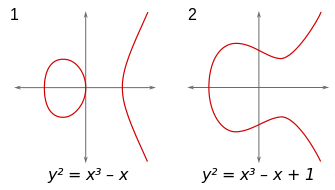
\includegraphics[width=.8\textwidth,center]{commonEC}
    \caption{Tipiche rappresentazioni di curve ellittiche}
\end{figure}
\begin{center}
\textbf{Point Addition}
\end{center}
Con il termine``Point Addition" si fa riferimento alla somma di due punti sulla curva costituisce la legge di gruppo per le curve ellittiche e viene definita come segue: 
\\
Dati due punti distinti $K$-razionali $A$ e $B$ sulla curva possiamo definire in modo univoco un terzo punto $C(x_C, y_C)$ dato dall'intersezione della retta passante per $A$ e $B$ e la curva. Il punto opposto $-C(x_C, -y_C)$ rappresenta la somma dei due punti: $A + B = B+ A = -C$. Il risultato dell'equazione $A+B+C = 0$ \`e il punto all'infinito. Il motivo di tale risultato \`e che la curva ellittica ha un singolo punto all'infinito il quale \`e un punto di flesso. Si pu\`o aggiungere che la linea all'infinito incontrer\`a una sola volta la curva, precisamente nel punto all'infinito, quindi tale punto determina un'intersezione di molteplicit\`a tre.
\begin{figure}[H]
    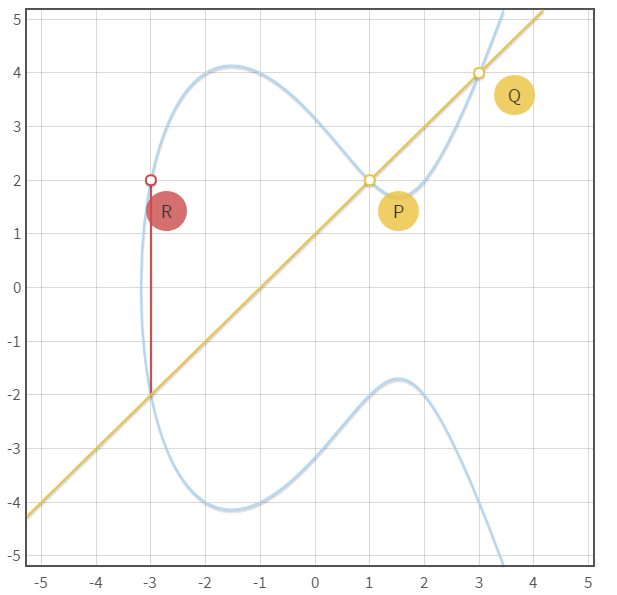
\includegraphics[width=.75\textwidth,center]{PA_P+Q}
    \caption{Point Addition sulla curva $y^2 = x^3-7x+10$}
\end{figure}

Esistono per\`o dei casi particolari:
\begin{enumerate}
    \item Somma di due punti simmetrici (opposti) tra loro $P$ e $Q = -P$. 
    \\
    Tramite il metodo della Point Addition si costruisce una retta per i due punti che risulta parallela all'asse y che andr\`a ad intersecare il punto all'infinito $O$. Definiamo quindi $P + Q = P+(-P) = O$,
    \begin{figure}[H]
        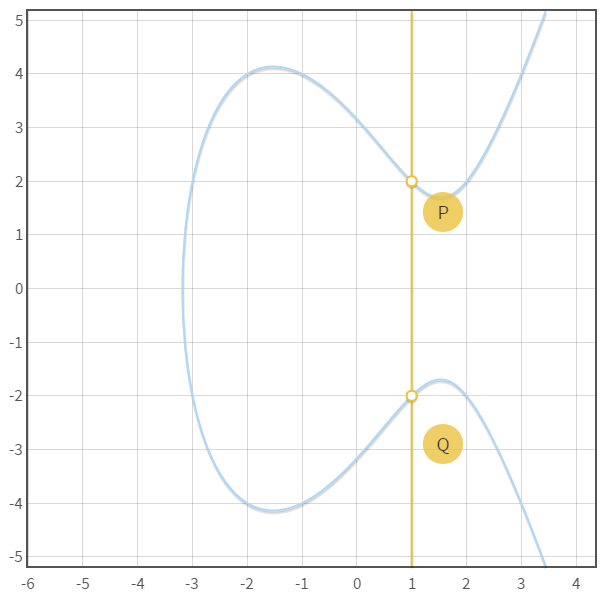
\includegraphics[width=.6\textwidth,center]{PA_P+(-P)}
        \caption{Curva $y^2 = x^3-7x+10$, $P=(1, 2)$, $Q=-P=(1, -2)$}
    \end{figure}
    \item Somma di un punto $P$ ed il punto all'infinito $O$. 
    \\ 
    La retta che unisce il punto $P$ ed il punto $O$ interseca la curva in un punto $Q = -P$, calcolando il punto $-Q$ otteniamo il risultato cercato ovvero $-(-Q) = P$.
    Ricordando che il punto $O$ viene trattato come elemento identit\`a del gruppo possiamo scrivere $P+O = O+P = P$,
    \item Somma di un punto $P$ e se stesso. 
    \\
    Non avendo due punti distinti non \`e possibile tracciare la retta per i due punti, immaginiamo quindi di prendere due punti ed avvicinarli uno all'altro sulla curva: la retta diventa tangente alla curva nel punto $P$, intercetta il punto $-Q$ ed il suo simmetrico \`e il risultato cercato: $P + P = Q$,
    \begin{figure}[H]
        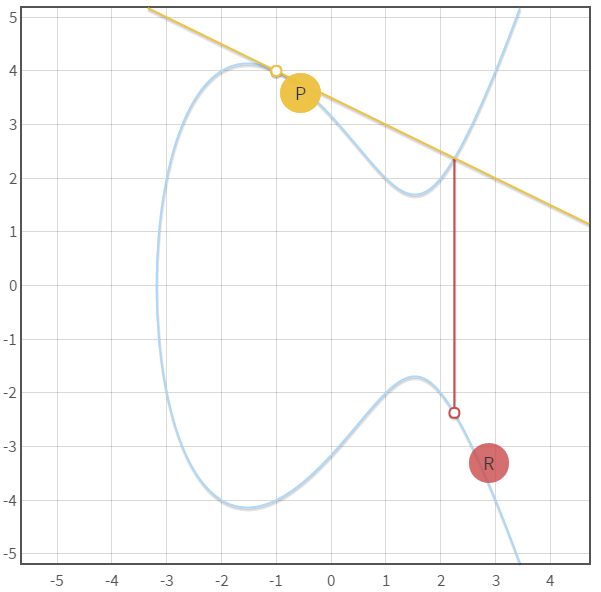
\includegraphics[width=.6\textwidth,center]{PA_P+P}
        \caption{Curva $y^2 = x^3-7x+10$, $P=Q=(-1, 4)$}
    \end{figure}
    \item Caso particolare: sommiamo $P+P$ ma tale punto \`e un flesso per la curva. 
    \\
    In un punto di flesso la concavit\`a della curva cambia ed in ogni curva ellittica esistono esattamente 9 punti di flesso. In questo caso consideriamo il secondo punto $Q =P$ e la somma finale viene ad essere $-P$, l'opposto del punto iniziale.
\end{enumerate}
Il calcolo del punto $C = A + B$ \`e dato per costruzione geometrica della retta $r$ passante per i punti $A(x_A, y_A)$ e $B(x_B, y_B)$. Detto $m$ il coefficiente angolare della retta $r_{AB}$, le coordinate del punto $C(x_C, y_C) = -(P+Q)$ saranno date dalle seguenti formule:
\begin{align*}
\begin{cases}
m = \ddfrac{y_A - y_B}{x_A - x_B}\\
x_C = m^2 - (x_A + x_B)\\
y_C = m(x_A - x_C)-y_A
\end{cases}
\end{align*}
%Aggiungi C = A + A e formule corrette
Si noti che nel caso in cui $x_A = x_B$ si ottiene uno zero al denominatore, $m$ porterebbe quindi la tangente ad essere parallela all'asse y ed il punto individuato dalla formula sarebbe il punto all'infinito $O$ per cui otterremmo $C = O$ esattamente come anticipato nel Caso Speciale 1.
\\
Come gi\`a visto, se vale $x_A = x_B$ abbiamo dei casi particolari per cui se $y_A = -y_B$ allora i due punti sono simmetrici e la loro somma \`e il punto all'infinito, se invece abbiamo $y_A = y_B = 0$ abbiamo che il punto $A$ ed il punto $B$ coincidono e si trovano all'estremit\`a sinistra della curva. La loro somma \`e ancora il punto all'infinito. Tuttavia esiste un altro caso particolare in cui si verifica $x_A = x_B$ ma $y_A = y_B \ne 0$, tale caso \`e detto \textit{Point Doubling}.
\\
\\
\begin{center}
\textbf{Point Doubling}
\end{center}
L'operazione del Point Doubling permette di sommare un punto a se stesso, se la sua ordinata $y$ \`e diversa da zero, ed ottenere un secondo punto sulla curva. Dato un punto $A(x_A, y_A)$ con $y_A \ne 0$ sommare $A+A$ equivale a trovare il punto $B = -(A+A) = -2A$. Quella che nel Point Addition era una retta per due punti diventa ora la tangente alla curva $y^2 = x^3 + ax +b$ nel punto $A$. La motivazione che ci porta ad usare la retta tangente alla curva viene dalla considerazione che presi due punti $P$ e $Q$ della curva, man mano che $Q$ si avvicina a $P$ pi\`u la curva tra i due punti tende a diventare la tangente. Le equazioni che permettono il calcolo del punto $B$ sono:
\begin{align*}
\begin{cases}
m = \ddfrac{3{x_A}^2 + a}{2y_A}\\
x_C = m^2 - 2x_A\\
y_C = m(x_A - x_C)-y_A
\end{cases}
\end{align*}
Si noti come il coefficiente angolare $m$ dipenda non solo dalle coordinate di $A$ ma anche dal coefficiente $a$ presente nell'equazione della curva. Tale formulazione discende dalla derivata prima dell'equazione della curva per cui si ha:
\begin{align*}
\ddfrac{d}{dx}y^2 &= \ddfrac{d}{dx}x^3 + ax + b\\
2y\ddfrac{d}{dx} &= 3x^2 + a\\
m = \ddfrac{d}{dx} &= \ddfrac{3x^2 + a}{2y}
\end{align*}
Quanto detto finora si applica a curve ellittiche nel campo dei numeri reali $\mathbb{R}$, tuttavia possiamo estendere il discorso ai numeri razionali $\mathbb{Q}$ in quanto definiti sul campo dei reali. La legge di gruppo (Point Addition) tra punti con coordinate reali si applica anche al campo $\mathbb{Q}$; le formule usate mostrano che la somma di due punti $A, B \in \mathbb{Q}$ comporta $C = A + B, \to C \in \mathbb{Q}$ dato che la retta $r_{AB}$ \`e a coefficienti razionali. In tal modo si dimostra che l'insieme di punti razionali della curva forma un sottogruppo del gruppo a punti reali. Essendo quest'ultimo un gruppo abeliano, tale sar\`a anche il sottogruppo dei numeri razionali; si conclude quindi che vale $C = A+B = B+A$.
\\
\\
Studiare una curva ellittica su di un campo finito (ovvero il numero dei suoi elementi \`e finito) porta la curva ad una``scomposizione" in punti, anch'essi in numero finito, perdendo la tipica forma vista negli esempi precedenti. L'equazione che governa la curva cambia leggermente: consideriamo $(x, y) \in \mathbb{Z}/p\mathbb{Z}$ con $p$ un numero primo\\
\begin{center}
$\begin{cases}
y^2 = x^3 + ax+b $ mod$(p)\\
4a^3 \ne 27b^2$ mod$(p)
\end{cases}
\bigcup $ $\{O\}$.\\
\end{center}
Il numero di elementi di una curva ellittica in un campo finito \`e difficile da determinare ma possiamo limitare in un intervallo tale cardinalit\`a grazie al teorema di Hasse sulle curve ellittiche: detti $K$ un campo finito con un $q$ elementi, $E$ una curva ellittica definita su tale $K$ e $cardE_K$ la cardinalit\`a (numero di elementi) della curva, possiamo dire che
\begin{align*}
    \mid cardE_K - (q+1) \mid \le 2 \sqrt{q}
\end{align*}
che ci porta a delimitare la cardinalit\`a tra i valori 
\begin{align*}
    q+1-2 \sqrt {q} \le cardE_K \le q+1+2 \sqrt {q}
\end{align*}
Consideriamo degli esempi: per un campo $K$ di $q=4$ elementi abbiamo una curva $E$ con $1 \le cardE_K \le 9$, $q=16 \to 9 \le cardE_K \le 25$, $q=64 \to 33 \le cardE_K \le 97$, $q=256 \to 129 \le cardE_K \le 385$. \`E importante notare che il teorema usato resituisce la cardinalit\`a della curva includendo il punto all'infinito.
Questi risultati ci portano ad affermare che il numero di elementi della curva \`e vicino al numero di elementi del campo. 
\\
Una curva con cardinalit\`a pari ad un numero primo \`e detta``curva prima".
\\
\\
\textbf{Considerazioni personali}: \textit{per numeri $q$ quadrati perfetti si pu\`o semplificare la formula di Hasse in ``$ \ddfrac{1}{2}q +1 \le cardE_K \le \ddfrac{3}{2}q +1$". Questa formula \`e stata trovata dall'osservazione dei risultati degli esempi precedenti e messa a confronto con numeri``non quadrati perfetti" come ad esempio un numero primo. La formula mostrata fornisce una stima coerente con quella di Hasse per``quadrati" ma fornisce una stima peggiorativa in tutti gli altri casi. Esempio: $q=160$, per Hasse abbiamo $136 \le cardE_K \le 186$, per la formula ideata abbiamo $81 \le cardE_K \le 241$}. 
\begin{figure}[H]
    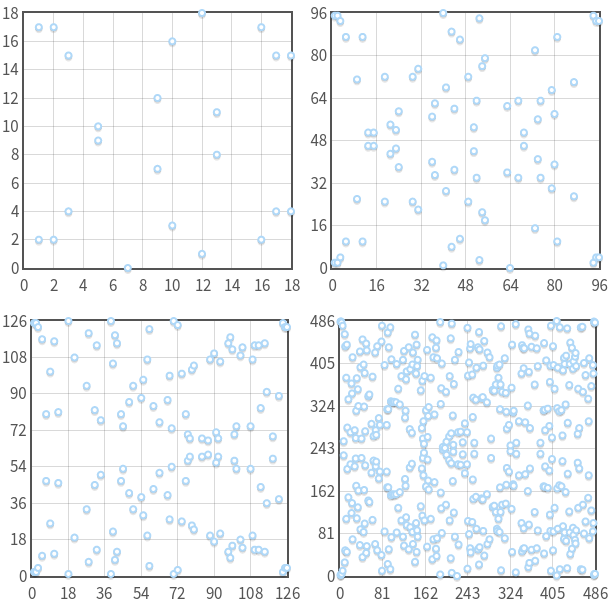
\includegraphics[width=.8\textwidth,center]{ECmod(p)}
    \caption{Curva $y^2 = x^3-7x+10$ mod $(p)$, $p = \{19, 97, 127, 487\}$}
\end{figure}
L'insieme di punti di $E$ per il campo dato $K_p$ \`e un gruppo abeliano finito, \`e inoltre un gruppo ciclico o il risultato di un prodotto tra due gruppi ciclici. Un esempio \`e dato dalla curva $y^2 = x^3 - x$ sul campo $K_{71} = \mathbb{Z}/2\mathbb{Z}\times\mathbb{Z}/36\mathbb{Z}$ che comprende un totale di 72 punti di cui 71 sono punti affini, incluso il punto $(0,0)$ ed uno \`e il punto all'infinito.
Numerosi algoritmi permettono il calcolo preciso del numero di punti per una curva ellittica su un campo finito; ad esempio l'algoritmo di Schoof parte dal teorema di Hasse, definisce $t = q+1-cardE_K$ e si procede nel calcolare la cardinalit\`a di ``$t\%N$" (operazione modulo), dove $N > 4\sqrt{q}$, tramite il teorema cinese del resto. La complessit\`a di questo algoritmo \`e pari a $O(n^{5+o(1)})$.
\\
%Altri algoritmi
%1 - https://en.wikipedia.org/wiki/Counting_points_on_elliptic_curves
%2 - https://en.wikipedia.org/wiki/Elliptic_curve#Elliptic_curves_over_finite_fields
%
\\
Risulta evidente che la curva abbia perso la sua tipica forma e di come sia composta di soli punti sparsi sul piano $xy$. 
\textbf{L'asse di simmetria} non \`e pi\`u $y=0$ ma \textbf{diventa} $\mathbold{y=p\big / 2}$, le operazioni studiate precedentemente non cambiano nonostante ci troviamo in presenza di un campo modulare. Le rette usate per la Point Addition e la Point Doubling non sono cambiate concettualmente, ma una differenza grafica notevole \`e che trovandoci in un campo modulare $p$ sono permesse coordinate con valori compresi tra $0$ e $p-1$, quei punti che escono fuori da questo intervallo vengono riportati in modulo $p$ sul grafico, lo stesso concetto si applica alla retta per cui viene ripetuta ciclicamente
\begin{figure}[H]
    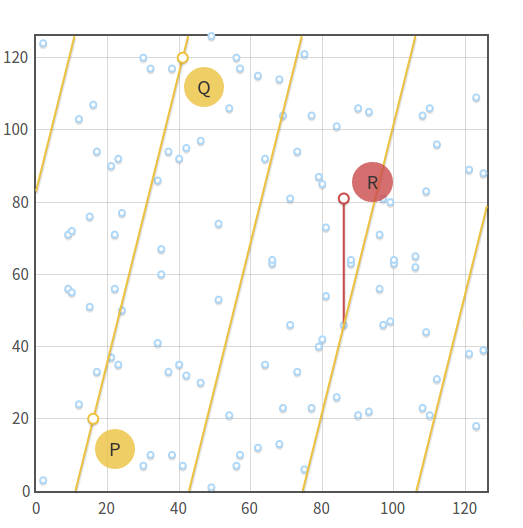
\includegraphics[width=.6\textwidth,center]{ECmodPA}
    \caption{Curva $y^2=x^3-x+3$ mod$(127)$, punti $P = (16, 20)$, $Q=(41, 120)$, $R = -(P+Q) = (86, 81)$ Cardinalit\`a: 111 elementi}
\end{figure}
Quanto velocemente riusciamo a calcolare il punto $nP$? Poniamo il caso di dover calcolare $n=100$, tramite ripetute Point Addition abbiamo il punto $P$ di innesco e dobbiamo computare i successivi 99 punti per trovare $100P$ per un totale di $n-1$ addizioni. Velocizzare questo risultato diventa davvero facile se pensiamo di usare un insieme di Point Addition (Add) e Point Doubling (Double): $n=1 \to A$, Double $\to n=2$, Add $\to n=3$, Double $\to n=6$, Double $\to n=12$, Double $\to n=24$, Add $\to n=25$, Double $\to n=50$ ed infine Double $n=100$ per un totale di 8 operazioni (6 Point Doubling e 2 Point Addition). Abbiamo ridotto notevolmente il numero di operazioni necessarie per raggiungere il coefficiente $n$. 
\\
L'uso di una notazione base $B$ aiuta a trovare un algoritmo efficiente per questi calcoli; partiamo dal considerare $100_{10} = 1100100_2 = d_6d_5d_4d_3d_2d_1d_0$ ed usiamo il seguente algoritmo: scorriamo il numero in base $B=2$ da sinistra verso destra ed usiamo l'operazione Point Doubling, nel caso di dover calcolare un $1$ facciamo seguire una Point Addition. 
\\
\\
Passo 0: $n=1_2 \to nP = P$. Il primo numero da trovare sar\`a sempre 1\\
Passo 1: Double $n \to 2n = 10_2$, dato che $d_5 = 1$ dobbiamo proseguire con una Add;\\
Passo 2: Add    $2 \to 3 = 11_2$. Procediamo quindi al calcolo degli altri $d_i$;\\
Passo 3: Double $3 \to 6 = 110_2$\\
Passo 4: Double $6 \to 12 = 1100_2$\\
Passo 5: Double $12 \to 24 = 11000_2$, dobbiamo avere $d_2 = 1$ quindi...\\
Passo 6: Add    $24 \to 25 = 11001_2$\\
Passo 7: Double $25 \to 50 = 110010_2$\\
Passo 8: Double $50 \to 100 = 1100100_2$\\
\\
Usando le operazioni indicate troviamo il punto cercato $100P$. Confrontiamo ora i costi computazionali dei due metodi visti. 
\\
Il primo consiste nel sommare $n-1$ volte lo stesso punto per arrivare al nostro $nP$; prendiamo il numero $n-1$ ed espresso in termini binari, base 2, vediamo che $n_2$ \`e formato da $k$ cifre $d_kd_{k-1} \ldots d_1d_0$. Il costo di $n-1$ addizioni \`e pari a $O(n-1)$ ed abbiamo visto che non \`e affatto un buon risultato. 
\\
Il secondo metodo, detto Double and Add, necessita di sole $O(log n)$ operazioni, dandoci un risultato nettamente migliore.
\\
\\
Data la curva $E: y^2 = x^3 +2x +2$ mod$(17)$ e dato il punto $A = (5, 1)$, usiamo la tecnica del Point Doubling per trovare il punto $2A$.
I dati che ci servono sono $a = 2$, coefficiente di $x$ nella curva, e le coordinate del punto $A$; passiamo alle formule:
\\
\\
$m = \ddfrac{3{x_A}^2 + a}{2y_A}= \ddfrac{3 \cdot 5^2 + 2}{2 \cdot 1} = \ddfrac{9}{2} \text{ mod}17= 9 \cdot 9 \text{ mod}17 = 13\text{ mod}17\\
x_C = m^2 - 2x_A= 13^2 - (2 \cdot 5) = 169\text{ mod}17 = 6 \text{ mod}17\\
y_C = m(x_A - x_C)-y_A= m(5 - 6)-1 = -14\text{ mod}17 = 3\text{ mod}17
$
\\
\\
Il punto trovato ha coordinate $2A = (5, 1)+(5, 1) = (6, 3)$.
\\
\begin{figure}
    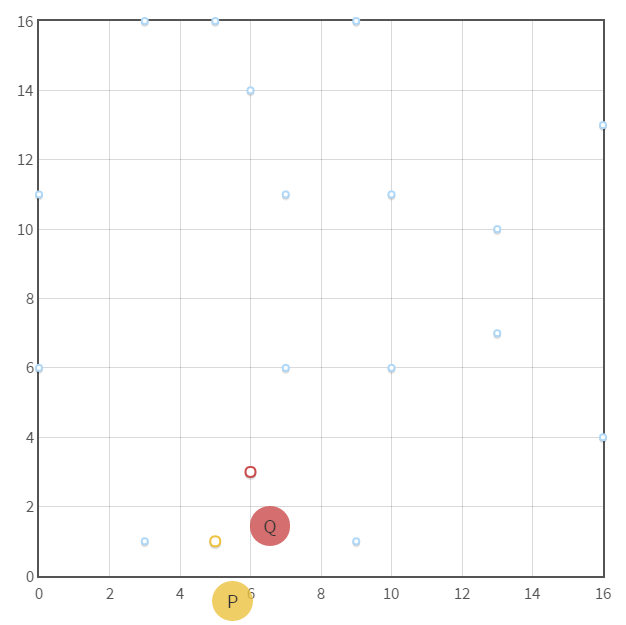
\includegraphics[scale=0.5, center]{PD_mod(17)}
    \caption{Curva $y^2=x^3+2x+2$ mod$(17)$, punto $P = (5, 1)$, $Q=2P = (6, 3)$}
\end{figure}
Come si nota dal grafico, i punti rappresentati sono in numero limitato. La cardinalit\`a secondo il teorema di Hasse \`e compresa nell'intervallo $[10, 26]$, se ci riferiamo alla figura e contiamo i punti rappresentati notiamo che questi sono in totale 19, compreso il punto all'infinito. Il risultato teorico rispetta il valore effettivo trovato.
\\
\`E possibile fare un'ulteriore verifica del risultato contando i punti tramite una Point Addition nel seguente modo: sappiamo che partendo dal punto $A(5, 1)$ abbiamo trovato $2A = (6, 3)$; possiamo quindi sommare i due punti trovati ed ottenere $3A = 2A + A = (10, 6)$. Procedendo analogamente troviamo $4A = (3, 1)$, $5A = (9, 16)$, $6A = (16, 13)$, $7A = (0, 6)$, $8A = (13, 7)$, $9A = (7, 6)$, $10A = (7, 11)$, $11A = (13, 10)$, $12A = (0, 11)$, $13A = (16, 4)$,  $14A = (9, 1)$, $15A = (3, 16)$, $16A = (10, 11)$, $17A = (6, 14)$, $18A = (5, 16)$, $19A = O$.
\\
Il punto $19A$ rappresenta il punto all'infinito.
Alcune considerazioni sui risultati ottenuti:
\begin{enumerate}
    
    \item Ancora una volta sono state rispettate le aspettative teoriche sulla cardinalit\`a della curva, abbiamo infatti trovato 19 punti distinti sulla curva.
    
    \item $19A$ \`e il punto all'infinito perch\`e corrisponde alla Point Addition $(5, 1) + (5, 16)$. L'ascissa \`e $5$ per entrambi i punti e l'ordinata \`e diversa da zero, i due punti sono quindi distinti sulla curva e, come gi\`a detto durante lo studio della Point Addition, il risultato deve essere il punto $O$ all'infinito.
    
    \item La somma di $A + 18A$ \`e il punto $19A = O$ ma lo stesso risultato lo si pu\`o ottenere sommando altri due punti come $2A + 17A$, $3A + 16A$, $4A + 15A$ e cos\`i via ottenendo sempre lo stesso risultato (lo si nota facilmente considerando che le ascisse delle coppie di punti dati sono le stesse).
    
    \item \textit{Considerazioni personali}: il calcolo dei 19 punti ha portato alla luce una ricorsivit\`a nei valori delle ascisse, i primi 9 punti hanno ascissa nella sequenza $5, 6, 10, 3, 9, 16, 0, 13, 7$ mentre i successivi 9 hanno ascissa in sequenza invertita. Due punti successivi tra loro presentano la stessa ascissa: $9A$ e $10A$, la loro somma \`e $19A = O$. 
    %Partendo da questo risultato \`e forse possibile trovare``facilmente" la cardinalit\`a di una curva? 
    \\
    \`E possibile affermare``calcolati due punti $nA$ e $(n+1)A$ di una curva $E$ su un campo finito $K$ tramite la legge di gruppo Point Addition, se vale $x_n = x_{n+1}$ allora il $nA + (n+1)A$ corrisponde al punto all'infinito e la somma delle molteplicit\`a dei due punti costituisce la Cardinalit\`a, per cui $cardE_K = n+(n+1) = 2n+1$"?
    \\
    La risposta \`e in generale``no". Quanto appena affermato non vale all'interno di gruppi``grandi"; prendiamo ad esempio la curva $y^2 = x^3 + 2x+3$ nel campo $\mathbb{Z}/97\mathbb{Z}$, con punto di partenza $P(3, 6)$. La curva ha in totale 100 punti ma il punto $P$ da noi considerato genera un sottogruppo, per il quale viene detto \textit{Generatore}, con meno di 100 punti. I punti sono $P(3, 6), 2P(80, 10), 3P(80, 87), 4P(3, 91), 5P = O$ da cui deduciamo che la cardinalit\`a di questo sottogruppo \`e 5, vale inoltre $2P+3P = 5P \to card(E_K) = 5$ in quanto $2P$ e $3P$ sono punti successivi tra loro con medesima ascissa; la ricorsivit\`a delle ascisse vista precedentemente si mantiene valida nel sottogruppo per cui possiamo scrivere ogni punto $kP$ come $(k$ mod $card(E_K))P$.\\
    Abbiamo infine provato che diversi punti di innesco generano diversi sottogruppi, ognuno con una sua cardinalit\`a $card(S_E) \le card(E)$ (nota: viene rispettata l'uguaglianza tra i due termini quando non esistono sottogruppi, esattamente come accadeva nel primo esempio). 
    
\end{enumerate}
L'ordine del punto $P$ \`e analogo al concetto di caratteristica $char(K)$ di un campo $K$ ovvero corrisponde al pi\`u piccolo numero intero positivo tale che $nP = 0$. L'ordine di $P$ \`e direttamente collegato alla caratteristica della curva ellitta per mezzo del \textit{Teorema di Lagrange} che afferma``la cardinalit\`a di un sottogruppo $H$ del gruppo $G$ \`e un divisore intero della cardinalit\`a di $G$"; in altri termini se il gruppo $G$ ha cardinalit\`a $N$ ed uno dei suoi sottogruppi ha cardinalit\`a $n$ allora $n$ \`e un divisore intero di $N$. Detto ci\`o possiamo costruirci un metodo per trovare la cardinalit\`a di un sottogruppo $H$ dato il punto generatore $P$: calcoliamo $N = card(E_K)$ tramite l'algoritmo di Schoof, prendiamo tutti i divisori interi di $N$ trovando quindi $n_1$, $n_2 \ldots$. Il pi\`u piccolo $n_x$ per cui verifichiamo $n_xP = 0$ corrisponde alla cardinalit\`a del sottogruppo.
\\
Esempio: la curva $y^2 = x^3-x+3$ mod$(37)$ ha cardinalit\`a $N=42$ per cui i suoi sottogruppi possono avere cardinalit\`a pari a $n= \{1, 2, 3, 6, 7, 14, 21\}$. Dato il punto $P=(2, 3)$ troviamo che la cardinalit\`a del sottogruppo $H_P$ \`e pari a 7 perch\`e $7P = 0$. Ovviamente anche $n = 14$, $n = 21$ ed $n=42$ portano a rispettare l'equazione $n_xP=0$ ma solo il divisore pi\`u piccolo corrisponde alla cardinalit\`a del sottogruppo.
\\
\\
\textbf{Ulteriore esempio}: curva $E: y^2 = x^3 -x+1$ mod$(29)$ ha cardinalit\`a $N=37$, un numero primo. I divisori di un numero primo sono solo $1$ e se stesso per cui la cardinalit\`a dei sottogruppi $H_G$ pu\`o essere o $1$ o $37$, tuttavia non possiamo accettare una cardinalit\`a $n=1$ in quanto ricordiamo che tale sottogruppo comprenderebbe solo il punto all'infinito. Deduciamo quindi che $n = N = 37$ \`e l'unico valore accettabile per la cardinalit\`a dei sottogruppi $H_G$ e che \textbf{esiste un solo sottogruppo $H$} corrispondente al gruppo generatore $G$ e comprendente tutti i punti della curva.
\\
Sempre come conseguenza del teorema di Lagrange possiamo individuare un numero $h= N \big / n, \mid h \in \mathbb{Z}$ che chiamiamo \textbf{cofattore del sottogruppo}. \`E importante notare che per ogni punto della curva viene verificata la seguente uguaglianza $NP=0$ poich\`e $N$ sar\`a sempre un multiplo di $n$, euesto ci permette di scrivere $n(hP)=0$. Supponiamo che $n$ sia un numero primo, l'equazione lascia quindi pensare che il punto $G = hP$ sia un generatore di un sottogruppo di cardinalit\`a $n$.
\\
Trovare un sottogruppo con la cardinalit\`a pi\`u grande possibile:
\begin{enumerate}
    \item Data la curva ellittica $E$ calcolare $N = Schoof(E)$ per ottenerne la cardinalit\`a;
    \item Calcoliamo il divisore \textbf{primo} pi\`u grande di $N$;
    \item Calcoliamo $h = N \big / n$;
    \item Continuiamo a scegliere un punto casuale $P$ sulla curva finch\`e $G = hP = 0$. Quando troviamo un valore per cui $G \ne 0$ allora possiamo dire che $P$ \`e un generatore del sottogruppo $H$ di cardinalit\`a $n$ e cofattore $h$.
\end{enumerate}
In matematica non \`e solitamente difficile trovare un numero $k$ data l'equazione $Q = kP$, nelle curve ellittiche il discorso cambia notevolmente. Trovare il coefficiente $k$ viene considerato un problema Difficile per la matematica, il nome con cui ci riferiamo a questo \`e \textit{Logaritmo Discreto}.
\\
Questo problema \`e analogo al problema del logaritmo discreto usato con sistemi di crittografia quali Digital Signature Algorithm (DSA), lo scambio di chiavi Diffie-Hellman (D-H) e l'algoritmo ElGamal usato nella crittografia asimmetrica (chiave pubblica). Questi algoritmi sono caratterizzati dal trovare il numero $k$ dall'espressione esponenziale con modulo: $b = a^k$ mod$p$. 
\\
L'aggettivo``ciclico" viene dato per via degli insiemi finiti o sottogruppi ciclici usati dagli algoritmi. Notiamo per\`o che non \`e presente alcun logaritmo per le curve ellittiche: la denominazione proviene dalla conformazione con l'espressione appena vista. L'espressione per le curve ellittiche presenta una difficolt\`a computazionale ben superiore ai problemi logartmici discreti analoghi, si \`e pensato quindi di usare questo problema come base per un sistema di crittografia chiamato Crittografia Ellittica.
%
%
%
%
%
\chapter{Dalla crittografia asimmetrica a quella ellittica}
\textbf{INSERISCI BACKGROUND STORICO SULLE BASI DELLA CRITTOGRAFIA }
\begin{itemize}
    \item Cifrario di Cesare
    \item Crittografia simmetrica
    \item Problema del CODEBOOK (?)
    \item Crittografia asimmetrica con RSA
    \item Crittografia ellittica
\end{itemize}
\noindent\makebox[\linewidth]{\rule{\paperwidth}{0.4pt}}
\\
\\
Il sistema a chiave asimmetrica (o pubblica) RSA \`e il pi\`u noto, si pu\`o usare anche per autenticazione e per garantire integrit\`a dell'informazione.
\\
La scelta delle chiavi pubblica e privata avviene nel seguente modo:
1. Scegliere casualmente due numeri primi, ``p" e ``q"
(tanto pi\`u grande sar\`a il loro valore tanto pi\`u difficile
risulter\`a violare RSA: si raccomanda che il prodotto di p
e q sia dell'ordine di 1024 o 2048 bit (con 1024 bit si
pu\`o rappresentare un numero con oltre 300 cifre)
2. Calcolare n = pq e z = (p-1)(q-1)
3. Scegliere un numero e (encryption), tale che : e<n, e>2 e che non abbia fattori in comune con ``z"
4. Scegliere un numero d (decryption), tale che d<n, ed – 1 sia un multiplo di ``z" (in altri termini, tale che il resto della divisione ed/z sia 1)
La chiave pubblica  ``KP" \`e la coppia (n, e) , la chiave privata ``KS" \`e la coppia (n, d) : B vuole inviare ad A un numero m, tale che m<n
• Per codificarlo, B usa la chiave pubblica di A KP=(n, e) per calcolare il messaggio cifrato ``c," dove ``c,"  = me mod n
• Per decifrare il messaggio ricevuto, A usa la propria chiave privata KS per calcolare m = cd mod n
• La scelta di ``e" e ``d `` garantisce che (me mod n)d mod n = m 
Perch\`e funziona RSA? – (me mod n)d mod n = (me)d mod n = med mod n
– Teorema: se p e q sono primi, e n = pq, allora: xy mod n = xy mod (p-1)(q-1)
– Applicando questo risultato, possiamo scrivere: med mod n = med mod (p-1)(q-1) mod n
– Ricordiamo che e e d sono stati scelti tali che ed – 1 sia divisibile per (p-1)(q-1) o, equivalentemente, che il resto di (p-1)(q-1)/ed sia 1- Cos\`i ed mod (p-1)(q-1) = 1
– Dato che m<n, abbiamo: m(ed mod (p-1)(q-1)) mod n = m1 mod n = m - Cos\`i abbiamo il risultato che volevamo:
med mod n = m (Cio\`e, cifrando un messaggio m con c=me mod n e decifrandolo con cd mod n otteniamo il messaggio iniziale)
Efficacia di RSA:
– Non si conoscono algoritmi veloci per la fattorizzazione dei numeri interi
– Quindi, pur conoscendo il numero n, \`e computazionalmente  proibitivo calcolare i fattori p e q .Per es., per fattorizzare un numero di 663 bit (200 cifre) un
gruppo di ricerca ha impiegato tre mesi usando un cluster di 80 computer (equivalente a oltre 55 anni con un computer solo) – Se venisse scoperto un algoritmo veloce per la fattorizzazione, il sistema RSA non sarebbe pi\`u sicuro
\\
\\
La crittografia ellittica si basa su sei parametri:
\begin{itemize}
    \item \textbf{p}, numero primo, specifica la cardinalit\`a del campo $\mathbb{Z}/p\mathbb{Z}$;
    \item \textbf{a}, \textbf{b} coefficienti nell'equazione breve di Weierstrass della curva ellittica;
    \item \textbf{G} il generatore del sottogruppo
    \item \textbf{n}, numero primo, rappresenta l'ordine di tale sottogruppo
    \item \textbf{h} il cofattore.
\end{itemize}
\textbf{Nota sull'importanza dei sottogruppi propri}: una curva ellittica $E$ definita su un campo $\mathbb{F}_p$, viene detta \textbf{anomala} se la cardinalit\`a $card(E) = p$. Per curve anomale sono stati descritti algoritmi come quello di Smart o Samaev che riescono a risolvere il problema del logaritmo discreto in tempo $O($ln $p)$.
\\
\\
Come possiamo definire una curva crittograficamente \textit{sicura}?
\\
Per rispondere alla domanda possiamo avvalerci di un ulteriore parametro: il seed $S$, un numero casuale che pu\`o essere utilizzato per generare o i coefficienti $a$ e $b$ o il generatore $G$ oppure entrambi. Generare questi parametri \`e possibile dal calcolo dell'hash di $S$
\begin{center}
    $S = random[min, max] \to H = hash(S) \to 
    \begin{cases}
        a = f(H)\\
        b = g(H)
    \end{cases}$
\end{center}
Viene cos\`i descritto un procedimento semplice da usare ma che risulta difficile nel caso di dover trovare il seed $S$ a partire dai coefficienti:
\begin{center}
$
\begin{cases}
    h_1 = f^{-1} (a)\\
    h_2 = g^{-1} (b)
\end{cases}$ se 
$h_1 = h_2 \Rightarrow H=h_1=h_2 \nrightarrow S=hash^{-1} (H)$
\end{center}
Una curva generata grazie ad un seed viene detta \textbf{Verificabile Random} (\textit{Verifiably Random}). Il principio dietro la scelta di hash per generare parametri prende il nome di NUMS (\textit{Nothing Up My Sleeve}) assicurando che la curva non sia stata appositamente creata per lasciare esposte vulnerabilit\`a note.
\\
\\
\textbf{Crittografia ellittica}
\\
Chiave privata: numero intero, casuale, $d \in [1, n-1]$\\
Chiave pubblica: punto della curva $H = dG$\\
Conoscere $d$ e $G$ ci porta facilmente a calcolare $H$, tuttavia partire dai punti $H$ e $G$ trovare il numero $d$ significa risolvere il Problema del Logaritmo Discreto.
\\
\\
L'algoritmo ECDH \`e l'acronimo di Elliptic Curve Diffie-Hellman e si basa sull'accordo di una chiave. Detti Alice (\textit{A}) e Bob (\textit{B}) le parti in gioco, $M$ il messaggio che vogliono scambiarsi in modo sicuro, l'algoritmo si basa sui seguenti passi:
\begin{enumerate}
    \item Entrambi $A$ e $B$ generano le loro chiavi private e pubbliche. Alice avr\`a chiave privata $d_A = random(1, n-1)$, e pubblica $H_A = d_AG$; Bob avr\`a invece $d_B = random(1, n-1)$, e pubblica $H_B = d_BG$;
    
    \item Si passa allo scambio di chiavi pubbliche $H_A$ e $H_B$ attraverso un canale non sicuro. Un ipotetico mal intenzionato $C$ \`e il Man in the Middle che cerca di intercettare le chiavi pubbliche. Nonostante la possibilit\`a di recuperarle, trovare le chiavi private consiste nel risolvere il PdLD;
    
    \item Alice si trova ora in possesso della sua chiave privata $d_A$ e della chiave pubblica di Bob $H_B$; si passa dunque a calcolare il Segreto condiviso $S_A$ tramite la seguente: $S_A = d_AH_B$. Bob fa lo stesso trovando $S_B = d_bH_A$.
\end{enumerate}
Tale segreto condiviso si dimostra essere lo stesso sia per Alice che per Bob, infatti avendo detto che le curve ellittiche formano un gruppo abeliano, vale la propriet\`a commutativa per cui \`e valida la seguente:
\begin{center}
    $S_A = d_A \cdot H_B = d_A \cdot (d_B \cdot G) = d_B \cdot (d_A \cdot G) = d_B \cdot H_A = S_B$
\end{center}
Alice e Bob possono ora comunicare in modo sicuro usando una crittografia simmetrica a partire dal segreto $S$: la chiave pu\`o essere, ad esempio, la coordinata $x_S$ per crittografare i messaggi successivi.
\\
\\
Curve diverse portano a protocolli diversi: \textbf{secp256k1} usa i seguenti parametri 
\begin{itemize}
    \item \textbf{p} = $0x$FFFFFFFF FFFFFFFF FFFFFFFF FFFFFFFF FFFFFFFF FFFFFFFF FFFFFFFE FFFFFC2F = $2^{256} - 2^{32}-2^9-2^8-2^7-2^6-2^4-2^0$;
    
    \item \textbf{a} $=0$;
    
    \item \textbf{b} $=7$;
    
    \item \textbf{G} $= (x_G, y_G)$
    \\
    $x_G$ = $0x$79BE667E F9DCBBAC 55A06295 CE870B07 029BFCDB 2DCE28D9 59F2815B 16F81798,
    \\
    $y_G$ = $0x$483ADA77 26A3C465 5DA4FBFC 0E1108A8 FD17B448 A6855419 9C47D08F FB10D4B8;
    
    \item \textbf{n} = $0x$FFFFFFFF FFFFFFFF FFFFFFFF FFFFFFFE BAAEDCE6 AF48A03B BFD25E8C D0364141;
    
    \item \textbf{h} $ = 1$
\end{itemize}
Usando questa curva l'algoritmo sopra descritto Alice calcola:\\
$d_A$ = hex(random(1, n-1)) = $0x$CA26D640 64C04556 8BC087B7 73137390 D2D412D8 E85E3BBA 11E7A87A F02A460C,\\
$H_A = (x_A, y_A) = d_AG$,\\
$x_A$ = $0x$50F1D077 DE0807EB 17E45781 BAD7AC8A 85EFBE48 5DB3988F 546CF300 E50F4750,\\
$y_A$ = $0x$C5C0324A F29FE9CF 4FC0E305 EE406E4D CF1D6166 9877CA62 B16ADE01 2466C0C7;\\
\\
Bob invece:\\
$d_B$ = hex(random(1, n-1)) = $0x$8840D8F4 08C63786 693A58C3 431489FE 6452C91E 2BD85B5A A982EC04 82B7D965,\\
$H_B = (x_B, y_B) = d_BG$,\\
$x_B$ = $0x$D9852BD0 8856BF07 1FF719E4 2B8D4CB1 E82D66F5 B0CB00CF C6B62892 E1A8FFCD,\\
$y_B$ = $0x$C28B6FCA 34E247C8 32EE7C4F 55EC1DD5 150E6800 66BDFD86 1A8A26A7 724CE7E9;\\
\\\
ed il segreto condiviso sar\`a il punto di coordinate:\\
$S_A = d_AH_B = d_bH_A = S_B = (x_S, y_S)$,\\
$x_S$ = $0x$11F9892D 57C6EAAD B9DE6475 BBCA2204 01FEAA84 3B7A1DB1 3C44C348 C0FB92F1,\\
$y_S$ = $0x$89FC9ED0 FF4B1D91 3E4978EF DF23BAD8 947528E0 C4DDD00D C0119149 DD5C08ED.
\\
L'algoritmo appena visto assume talvolta la notazione ECDHE - ECDH Ephemeral facendo riferimento al fatto che le \textbf{chiavi pubbliche scambiate sono temporanee} e non statiche. Una volta stabilita la connessione tali chiavi effimere vanno validate da un ente certificato come ad esempio TLS/SSL.
\\
\\
\begin{center}
    \textbf{Firma Digitale}
\end{center}
Applicare una firma sulle chiavi \`e compito dell'ECDSA - Elliptic Curve Digital Signature Algorithm, diretta variante di un protocollo esistente (DSA) applicata alle curve ellittiche. L'idea della firma digitale si basa su Alice che vuole firmare un messaggio $m$ con la sua chiave privata $d_A$, successivamente Bob vorr\`a accertarsi di star parlando effettivamente con Alice e cercher\`a di validare la firma tramite la chiave pubblica di Alice $H_A$. La forza della firma digitale \`e che solamente Alice \`e in grado di generare una firma valida $F_A$ e tutti sono in grado di verificarne l'autenticit\`a grazie alla chiave \textbf{pubblica} $H_A$ necessaria alla verifica.
\\
ECDSA si basa sull'hash del messaggio $H = hash(m)$ piuttosto che sul messaggio in chiaro $m$.
\\
\\
\textbf{La scelta dell'hash}: l'algoritmo per produrre l'hash deve esser nell'ottica di una funzione crittograficamente sicura. In data 23 Febbraio 2017, Google ha completato l'esperimento``SHAttered" con il quale si mirava a trovare una collisione sull'algoritmo SHA-1. L'attacco portato avanti da Google ha richiesto la cifra di $9,223,372,036,854,775,808$ calcoli di SHA-1, utilizzando l'equivalente di 6500 anni di calcoli per una singola CPU, 110 anni di calcoli per una singola GPU, ottenendo il risultato di un attacco 100,000 volte pi\`u veloce di un attacco Brute Force normale.
\\
Sebbene ormai deprecato dal NIST nel 2011, molte applicazioni web e browser fanno ancora uso di SHA-1: Google Chrome ha preventivamente abilitato algoritmi pi\`u sicuri, Firefox ha ufficialmente deprecato SHA-1 solo nella versione 52 mentre Internet Explorer e GIT non hanno ancora pronta una patch. \\
GIT \`e un'applicazione che permette a gruppi di persone di lavorare assieme, da remoto, sullo stesso progetto; lo spazio di lavoro \`e detto \textit{Repository}. Il salvataggio dei dati si basa su``commit" generati da SHA-1 rendendo essenzialmente possibile creare due spazi di lavoro con lo stesso commit ma contenuti differenti. \`E sempre pi\`u valida l'idea di un utente malintenzionato che tramite un commit noto, crei un repository con annessa \textbf{Backdoor} ma stesso commit, scambi i due repository ed attacchi la vittima.
\\
\\
Scelto quindi un algoritmo sicuro, l'hash $H = hash(m)$ dovr\`a essere troncato ad $n$ bit; ricordiamo che $n$ corrisponde alla cardinalit\`a del sottogruppo generato dal punto $G$. Il nostro hash troncato \`e un numero intero e lo chiamiamo``$T$". La firma viene quindi generata secondo i seguenti passi:
\begin{enumerate}
    \item Si sceglie un numero $k = random(1, n-1)$, analogo alla Chiave Privata $d_A$;
    \item Si calcola il punto $P = (x_P, y_P) = kG$, analogo alla chiave pubblica $H_A$;
    \item Si calcola $r = x_P $ mod$(n)$;
    \item Se $r = 0$ (\`e un multiplo intero di $n$) si torna al punto 1;
    \item Si calcola $f = k^{-1} (T+rd_A) $ mod$(n)$, $k^{-1}$ \`e il moltiplicativo inverso di $k$ mod$(n)$;
    \item Se $f = 0$ (\`e un multiplo intero di $n$) si torna al punto 1.
\end{enumerate}
La coppia $F = (r, f)$ \`e la \textbf{firma}.
\\
Il segreto $k$ viene quindi usato per calcolare il punto $P$ e viene poi usato per generare $r$; infine si lega $r$ all'hash del messaggio tramite $f$. Trovare il segreto $k$ significa poter firmare messaggi fingendosi Alice ma il compito \`e difficile in quanto richiede di risolvere il noto Problema del Logaritmo Discreto.
\\
Come visto nell'algoritmo, $f$ deve essere diverso da $0$ e quindi non deve essere un divisore intero di $n$. \`E possibile utilizzare l'algoritmo solo se $n$ \`e un numero primo per \`e certo che $f$ sar\`a diverso da $0$. \textbf{Se il sottogruppo $H$ ha un ordine $n$ non primo, ECDSA non pu\`o essere utilizzato}, per questo motivo la maggior parte delle curve usate nella crittografia ellittica sono standardizzate e permettono numeri primi come cardinalit\`a $n$.
\\
\\
Bob \`e ora in possesso della firma $F = (r, f)$ di Alice e vuole verificarne l'autenticit\`a. Tramite i parametri noti quali il punto Generatore $G$, la cardinalit\`a $n$ del sottogruppo, la chiave pubblica $H_A$, l'hash troncato``$T$", la firma $F$, Bob procede come segue:
\begin{enumerate}
    \item Calcola il numero intero $u_1 = f^{-1}T$ mod$(n)$;
    \item Calcola il numero intero $u_2 = f^{-1}r$ mod$(n)$;
    \item Calcola il punto $P = u_1G + u_2H_A$.
\end{enumerate}
La firma $F$ viene quindi ritenuta valida se l'uguaglianza $r = x_P $ mod$(n)$ viene rispettata.
\\
Possiamo verificare la correttezza dell'algoritmo partendo dal punto $P$ e procedendo come segue:
\begin{align*}
    P &= u_1G + u_2H_A, &\text{ sostituiamo } H_A = d_AG\\
    &= u_1G + u_2d_AG, &\text{ raggruppiamo secondo G }\\
    &= (u_1 + u_2d_A)G, &\text{ sostituiamo } u_1 = f^{-1}T \text{ mod$(n)$, } u_2 = f^{-1}r\text{ mod$(n)$}\\
    &= (f^{-1}T + f^{-1}r \cdot d_A)G, &\text{ raggruppiamo secondo } f^{-1}\\
    &= f^{-1}(T + r \cdot d_A)G
\end{align*}
L'omissione, a sinistra, del``mod$(n)$" \`e volontaria in quanto $G$ ha cardinalit\`a $n$ per cui il risultato non cambia rendendo``mod$(n)$" superfluo.
\\
L'ultimo passo da fare \`e considerare la struttura di $f^{-1}$ ovvero $f = k^{-1} (T+rd_A)$ dalla quale troviamo che $k = f^{-1} (T+rd_A)$ per cui:
\begin{align*}
    P &= f^{-1}(T + r \cdot d_A)G, &\text{ sostituiamo quindi } k = f^{-1} (T+rd_A)
    &= kG
\end{align*}
Il valore trovato corrisponde a quello calcolato in fase di generazione della firma, come si pu\`o notare dal passo 2, per cui l'algoritmo funziona correttamente e l'autenticit\`a di Alice \`e confermata.
\\
\\
Tutti questi calcoli sono costruiti a partire dal segreto $k$ rendendolo molto importante per il corretto funzionamento dell'algoritmo. L'uso di un segreto $k$ statico induce l'indebolimento dell'algoritmo: la PlayStation3 legge solo giochi firmati con crittografia ECDSA e $k$ statico rendendo facile calcolare la chiave privata $d_S$ della Sony semplicemente avendo a disposizione due giochi firmati. Potendo rappresentare ciascun gioco con la tripla $(T, r, f)$, il procedimento per trovare la chiave privata $d_S$ della Sony \`e il seguente
\begin{align*}
     &r_1 = r_2 &\text{ in quanto $r = x_P = kx_G$}\\
     &f_1 - f_2 = k^{-1} [T_1+r_1d_S - (T_2 + r_2d_S)] &\text{ dalla $f = k^{-1} (T+rd_S)$}\\
     &f_1 - f_2 = k^{-1} (T_1 - T_2)  \text{ mod$(n)$} &\text{ $r_1d_S$ e $-r_2d_S$ si sono semplificati}\\
     &k= (T_1 - T_2)(f_1 - f_2)^{-1} \text{ mod$(n)$}
\end{align*}
Siamo quindi giunti a calcolare il valore di $k$ a partire dai due hash``$T$" e dai loro valori firmati $f$. Per estrarre quindi la chiave $d_S$ basta partire dall'equazione
\begin{align*}
     f &= k^{-1}(T+rd_S) \text{mod}(n) &\text{e ricavare la } d_S\\
     d_S &= r^{-1}(fk-T) \text{mod}(n) 
\end{align*}
Allo stesso modo \`e possibile calcolare chiavi private $d$ se il segreto $k$ \`e costruito in modo prevedibile.
%
%
%
%
%
%
%
%
%
%
%
%
%
%
%
\chapter{Attacchi alle EC}
Rompere la sicurezza delle curve ellittiche significa risolvere il Problema del Logaritmo Discreto ovvero: dati due punti $P$ e $Q$ di una curva ellittica definiti come $Q = xP$, dobbiamo riuscire a calcolare $x$. Un ulteriore dato necessario da ricordare \`e il punto generatore $G$ di un sottogruppo con cardinalit\`a $n$.
\\
\begin{center}
    \textbf{1. Baby Step, Giant Step}
\end{center}
L'idea dell'algoritmo si basa sulla considerazione che il numero cercato $x$ possa essere visto come somma di altri interi, infatti possiamo dire che $x = am+b$, $a, b, m \in \mathbb{Z}$ sono tre numeri interi arbitrari. Se $x$ fosse pari a 51 allora $x = 51 = 5 \cdot 10 + 1$. \`E quindi lecito scrivere:
\begin{align*}
    Q &= xP &\text{ Sostituiamo ora }x = am+b\\
    Q &= (am+b)P &\text{ Portiamo fuori dalle parentesi }\\
    Q &= amP+bP &\text{ Quindi portiamo a sinistra il termine }amP\\
    Q -amP &= bP
\end{align*}
Abbiamo trovato quindi due termini che possiamo calcolare allo stesso tempo e confrontare i risultati ottenuti; calcoliamo quindi i seguenti valori:
\begin{align*}
    &m = \ceil{\sqrt{n}} &\text{Arrotondato per eccesso}\\
    &bP \text{ }\forall b \in [0, m] &\text{Salviamo i risultati in una tabella di hash}\\
    &Q -amP \text{ }\forall a \in [0, m-1] &\text{Ripetere finch\`e } Q -amP \ne bP
\end{align*}
Quando usciamo dall'algoritmo possiamo dire di aver trovato la $x = am+b$ in quanto si \`e verificata l'uguaglianza $Q -amP = bP$.
\\
Il nome dell'algoritmo deriva dal fatto che vengono fatti piccoli passi (Baby Step) nei calcoli di $bP$ e grandi passi (Giant Step) quando calcoliamo $Q-amP$. Inoltre perch\`e abbiamo definito $m = \sqrt{n}$? La spiegazione si trova osservando l'equazione $Q = amP+bP$:\\
\\
$\begin{cases}
    a = 0 \to Q=amP+bP=0P+bP=bP &\Rightarrow [0P, mP]\\
    a = 1 \to Q=amP+bP=mP+bP &\Rightarrow  [mP, 2mP]\\
    a = 2 \to Q=amP+bP=2mP+bP &\Rightarrow  [2mP, 3mP]\\
    \ldots\\
    a = m-1 \to Q=amP+bP=(m-1)mP+bP &\Rightarrow  [(m-1)mP, m^2P]
\end{cases}$
\\
\\
Essendo vero che $m^2P=nP$ \`e evidente che abbiamo cercato in tutti i valori possibili ma con un numero contenuto di operazioni: esattamente $m$ moltiplicazioni per trovare tutti i $bP$ ed un massimo di altre $m$ operazioni per il confronto con $Q-amP$; l'algoritmo ha quindi una complessit\`a di tempo e spazio pari a $O(\sqrt{n})$.
\\
Abbiamo un netto miglioramento di prestazioni se paragonato ad un attacco Brute Force, tuttavia la sua applicazione resta resta ancora difficile; l'approccio usato dal BabyStep-GiantStep si basa su un tipo di attacco chiamato``meet-in-the-middle" in quanto prima dividiamo il problema in due parti e procediamo computando le due parti fino a trovarci``nel mezzo" del problema. Una curva standardizzata come secp192r1 presenta cardinalit\`a $n = $ 0x\textit{FFFFFFFF FFFFFFFF FFFFFFFF 99DEF836 146BC9B1 B4D22831}, il numero di operazioni sar\`a $m = \sqrt{n} \approx 7.9 \cdot 10^{28}$. La tabella di hash deve contenere dei punti di 32 bytes complessivi per un utilizzo di $32 \cdot 7.9\cdot 10^{28} \approx 2.5 \cdot 10^{30}$ bytes di memoria, un valore troppo grande da memorizzare.
\\
\begin{center}
    \textbf{2. La $\mathbold{\rho}$ di Pollard}
\end{center}
Un altro algoritmo per la risoluzione del Problema del Logaritmo Discreto \`e la $\rho$ di Pollard che presenta la stessa complessit\`a di tempo $O(\sqrt{n})$ del BSGS ma una complessit\`a di spazio pari a $O(1)$. Il problema consiste ora nel risolvere la forma $aP + bQ = AP + BQ$ dove $a$, $b$, $A$, $B$ sono numeri interi. Cerchiamo quindi di semplificare l'equazione:
\begin{align*}
    aP + bQ &= AP + BQ &\text{Sostituiamo il punto }Q = xP\\
    aP + bxP &= AP + BxP &\text{Portiamo a sinistra $AP$ ed a destra $bxP$}\\
    aP -AP &= BxP -bxP &\text{Raccogliamo il punto }P\\
    (a -A)P &= (Bx -bx)P &\text{Raccogliamo la x a destra}\\
    (a -A)P &= (B -b)xP &\text{Semplifichiamo $P$ ed aggiungiamo il mod$(n)$}\\
    a -A &= (B -b)x\text{ mod$(n)$} &\text{Evidenziamo la x}\\
    x &= (a -A)(B -b)^{-1}\text{ mod$(n)$}
\end{align*}
L'aggiunta del mod$(n)$ \`e dovuta al fatto che il sottogruppo considerato \`e ciclico di $n$ elementi totali, da questo deriva che anche i coefficienti usati nella Point Doubling/Addition sono considerati mod$(n)$.
\\
L'utilizzo di questa formula si basa sulla scelta di una \textbf{sequenza} di valori pseudo-casuali per la coppia $(a, b)$ con la quale generiamo la sequenza $aP+bQ$ e, dato che $P$ e $Q$ sono elementi di un gruppo ciclico, anche tutti i punti della sequenza $aP+bQ$ saranno ciclici. Questo ci porta a trovare un ciclo tale che le coppie $(a, b) \ne (A, B)$ conducano a $aP+bQ = AP+BQ$.
\\
Trovare il ciclo \`e un compito che possiamo svolgere con un algoritmo denominato``la Lepre e la Tartaruga": data la sequenza di $(a, b)$ calcoliamo la rispettiva sequenza di punti $aP+bQ$ e scorriamola a due velocit\`a differenti, la tartaruga T legger\`a ogni punto mentre la lepre L li legger\`a alternati, saltando un punto ad ogni passo. Confrontando i punti trovati da T ed L ad ogni passo arriviamo a trovare il ciclo cercato. Le operazioni necessarie richiedono complessit\`a spaziale $O($log$n)$ e temporale $O(\sqrt{n})$.
\\
Un'alternativa da non prendere in considerazione \`e quella di calcolare tutti i possibili valori per la coppia $(a, b)$ ovvero $n \cdot n = n^2$ coppie porta ad un costo di $O(n^2)$, non solo peggiore del BSGS ma addirittura di un attacco Brute Force.
\\
Per un esempio concreto dell'algoritmo $\rho$ di Pollard possiamo considerare un evento datato 2004 in cui Chris Monico riusc\`i a risolvere il Problema del Logaritmo Discreto su una curva di 109bit di lunghezza ed una versione migliorata dell'algoritmo della $\rho$ di Pollard. I calcoli effettuati da Monico hanno richiesto 17 mesi di tempo prima di risolvere il problema. 
\\
Possiamo fare stime su altre curve mediante una proporzione: con gli stessi strumenti di Monico, risolvere il logaritmo discreto per una curva a 192 bit con complessit\`a temporale $O(\sqrt{n})$ comporterebbe
\begin{center}
    $17$ mesi $\times \ddfrac{\sqrt{2^{192}}}{\sqrt{2^{109}}} = 17$ mesi $\times \sqrt{2^{83}} \approx 5 \cdot 10^{13}$ mesi\\
\end{center}
Nuove versioni di questo metodo portano ad un numero massimo di $\sqrt{\pi n \big / 4}$ operazioni risultando quindi nelle seguenti stime:
\begin{center}
\begin{tabular}{ c c c }
    n & Operazioni & Anni MIPS\\
    \hline
    $160$ &$2^{80}$ &$8.5 \cdot 10^{11}$\\
    $192$ &$2^{96}$ &$5.6 \cdot 10^{16}$\\
    $224$ &$2^{112}$ &$3.7 \cdot 10^{21}$\\
    $256$ &$2^{128}$ &$2.4 \cdot 10^{26}$\\
    $384$ &$2^{192}$ &$4.4 \cdot 10^{45}$\\
    $521$ &$2^{260}$ &$1.3 \cdot 10^{66}$\\
\end{tabular}
\end{center}
Nota su``Anni MIPS": La sigla MIPS indica``Million Instructions Per Second", con la notazione usata si intende sottolineare quanti anni sono necessari ad un calcolatore per computare tutte le operazioni assegnate se computa un milione di istruzioni al secondo.
\begin{center}
    \textbf{3. L'algoritmo di Shor}
\end{center}
L'algoritmo di Shor \`e nato per calcolare i fattori primi di un dato numero N, in termini di curve ellittiche: trovare il pi\`u grande fattore primo di $n$. \`E un algoritmo quantistico in grado di risolvere logaritmi discreti con complessit\`a temporale $O(($log $n)^3)$ e spaziale $O($log $n)$. L'efficienza di tale algorimo risiede nello \textbf{stato di superposizione} dei qubits, l'unit\`a quantica che rappresenta i bit, nel quale i qubit non hanno uno stato definito funch\`e non misurati; in altre parole quando misuramo un qubits abbiamo una certa possibilit\`a di osservare uno $0$ ed un'altra di osservare un $1$. Gli algoritmi quantici, come quello di Shor, lavorano modificando la probabilit\`a di ciascun bit.
\\
Sulla base di questa probabilit\`a \`e possibile computare numerosi input contemporaneamente avendo un numero limitato di qubit. Applicando questi concetti al logaritmo discreto per una curva ellittica abbiamo la possibilit\`a di trovare un numero $x$ distribuito in modo ciclico (uniforme) tra $0$ ed $n-1$ utilizzando ``$log(n)$" qubits invece di ``$n \cdot log(n)$" bits. Computare adesso il prodotto scalare $xP$ indurrebbe la superposizione per tutti i punti nell'intervallo $[0P, (n-1)P]$, misurare i qubits in questo momento ci farebbe ottenere uno di quei punti con probabilit\`a $1 \big / n$.
\\
L'algoritmo di Shor si basa quindi su questi concetti per calcolare $n$ stati alla volta, ridurli a pochi stati e quindi ottenere un \textbf{risultato unico} e non molti.
%
%
\\
\\
\\
\\1 - file:/.../TESI - ATTACCHI ALLE EC.pdf
%
%
%
%
%
%
%
%
\chapter{Livelli di sicurezza}
La sicurezza di una primitiva crittografica, algoritmo di basso livello sul quale costruire protocolli crittografici, si misura in base allo``\textit{sforzo per romperlo}". Se assumiamo che tale sforzo sia $2^k$ allora la primitiva offre una \textit{sicurezza a k-bit} e viene detta avere un \textbf{livello di sicurezza k}. Sistemi di crittografia simmetrica devono permettere una sicurezza di $k$-bit mediante una chiave della di $k$-bit; se questo principio non dovesse valere, il sistema non \`e da considerarsi``buono". Le funzioni di hash differiscono da quanto appena visto: un hash di lunghezza $l$ non pu\`o offrire pi\`u di $l \big / 2$ bit di sicurezza. 
\\
Conoscere il livello di sicurezza di una primitiva permette di rapportare e calcolare la sicurezza di algoritmi usati nella crittografia asimmetrica, come RSA e ECC, agli standard della crittografia simmetrica. Il tempo di computazione impiegato da RSA per generare la chiave pubblica pu\`o essere misurato mediante esperimenti oppure stimato: se fattorizzare un modulo da $n$-bit richiede un tempo $T_{RSA}$, il tempo richiesto per fattorizzare un modulo da $m$-bit (con $m>n$) \`e stimato come: 
\begin{center}
    $ \ddfrac{N(m)}{N(n)} \cdot T_{RSA}$, dove $N(k) = e^{1.923 \sqrt[3]{( \text{ln }2^k) \cdot ( \text{ln ln }2^k)^{2}}}$
\end{center}
Introduciamo gli algoritmi asimmetrici che fanno uso del logaritmo discreto: chiamiamo $G$ un gruppo di ordine $q$ tale che il tempo $T_{LD}$ per computare l'operazione di gruppo sia $T_{LD} = T_S \big / 2^c$, avendo indicato con $T_S$ il tempo richiesto da una applicazione di un sistema crittografico Simmetrico, ed avendo assunto che il parametro $c$ sia compreso nell'intervallo $0 \leq c \leq 10$. Risolvere il logaritmo discreto nel gruppo $G$ considerato offre ``$c+log_2(\sqrt{q})$"-bit di sicurezza. Ponendo il caso di una curva debole con $q$ pari ad un numero primo di 160 bit, il livello di sicurezza della curva assume il valore ``$c+80$".
\\
\`E possibile riassumere i livelli di sicurezza nei seguenti casi
\begin{enumerate}
    \item Sistemi crittografici simmetrici: pari alla lunghezza della chiave;
    \item Funzioni crittografiche di hash: pari a met\`a della lunghezza dell'hash;
    \item RSA: piccola e decrescente frazione della lunghezza del modulo;
    \item Logaritmo Discreto: pari alla met\`a di $n$ (che si ricorda essere il pi\`u grande numero primo divisore della cardinalit\`a del gruppo $G$).
\end{enumerate}
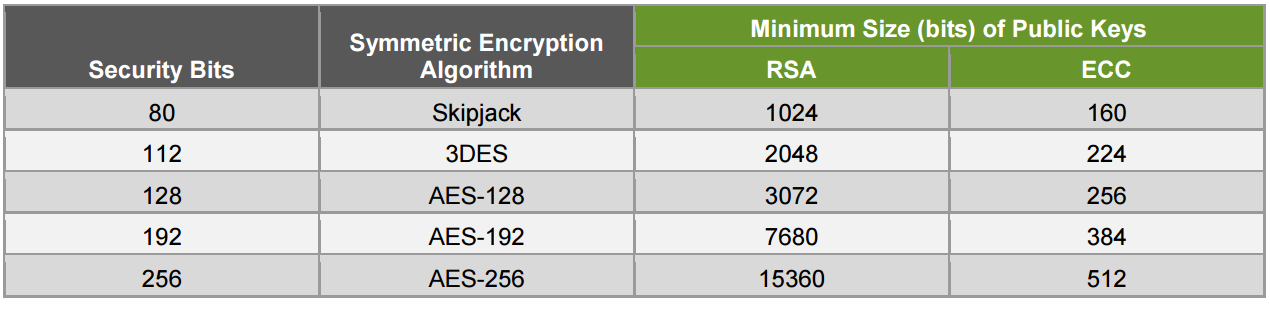
\includegraphics[scale=0.45]{RSAvECC_table}
\\
%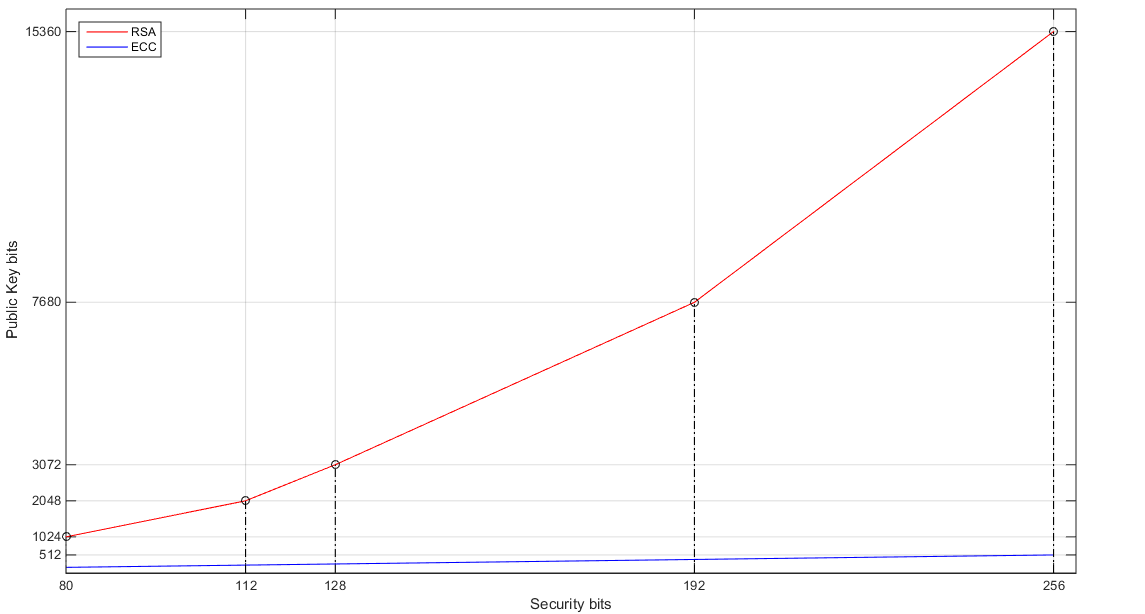
\includegraphics[scale=0.55]{RSAvECC_matlab}
%Il minor numero di bit per ECC rende l'algoritmo molto pi\`u veloce di RSA sia per la generazione delle chiavi che per la firma digitale. Il problema del logaritmo discreto per le curve ellittiche viene risolto da algoritmi molto pi\`u lenti di quelli usati per RSA.
L'importanza di chiavi``piccole" \`e fondamentale se consideriamo che moltiplicare due numeri molto grandi pu\`o causare una latenza eccessiva sui dispositivi meno performanti (come vecchi cellulari o tablet), al tempo stesso la sicurezza va aumentata con l'inevitabile aumento della lunghezza delle chiavi per RSA.
\\
L'ECC permette implementazioni sulle``\textbf{Smart Card}" per via della dimensione ridotta delle chiavi usate ed \`e l'unico sistema di crittografia possibile sulle carte \textbf{Contactless}: gli altri algoritmi richiedono troppa induzione di energia.
\\
Con ECC otteniamo risultati nettamente migliori di quelli offerti da RSA sia per la generazione di chiavi che per la firma digitale. 
Test benchmark sul calcolo della chiave pubblica: confrontiamo ECC-160bit contro RSA-1024bit, ECC-192bit contro RSA-1536bit, ECC-224bit contro RSA-2048bit evidenziando quante chiavi vengono generate al secondo con relativo commento sulle performance tra gli algoritmi 
\begin{align*}
    &\textbf{ECC}& &\textbf{RSA}& &\textbf{$\mathbold{k_{ECC}}$/s}& &\textbf{$\mathbold{k_{RSA}}$/s}& &\textbf{Efficienza}& &\textbf{Rapporto Chiavi}&\\
    &160& &1024& &271.3& &114.3& &2.4:1& &1:6.4&\\
    &192& &1536& &268.5& &36.4& &7.4:1& &1:8&\\
    &224& &2048& &195.5& &17.8& &21.4:1& &1:9.1&
\end{align*}
La notazione``\textbf{k/s}" intende esprimere la media di chiavi pubbliche generate al secondo.
\\
Test benchmark sulla firma digitale: usando un MacBook Pro ed OpenSSL 0.9.8 (versione non ottimizzata per ECDSA), generiamo firme ECDSA da 256bit e firme RSA da 2048bit; otteniamo i seguenti risultati
\begin{align*}
    &\textbf{ECC}& &\textbf{RSA}& &\textbf{$\mathbold{F_{ECC}}$/s}& &\textbf{$\mathbold{F_{RSA}}$/s}& &\textbf{Efficienza}& &\textbf{Rapporto Chiavi}&\\
    &256& &2048& &4287.4& &186.4& &23:1& &1:4&
\end{align*}
%\begin{align*}
%    &\text{Doing 256 bit sign ecdsa's for 10s:} &42874  %&\text{ 256 bit ECDSA signs in 9.99s}&\\
%    &\text{Doing 2048 bit private rsa's for 10s:} &1864 %&\text{ 2048 bit private RSA's in 9.99s}&
%\end{align*}
La notazione``\textbf{F/s}" intende esprimere la media di firme generate al secondo.\\
ECDSA risulta pi\`u di 20 volte pi\`u performante di RSA.
\\
\\
\textbf{Sicurezza della chiave privata}
\\
Ogni chiave privata deve esser generata in modo da non poter essere indovinate da utenti malintenzionati, si fa uso di un``\textbf{RNG} - \textit{Random Number Generator}" basato su rigide specifiche. Un RNG conserva il suo stato ``$\mathbold{s}$" e fornisce un output che deve essere il risultato di una \textit{funzione a senso unico} dello stato ``${rnd = f(s)}$" per assicurare che non si possa risalire allo stato a partire dall'output. Inoltre tale stato dovrebbe esser aggiornato con una diversa funzione a senso unico tale da impedire predizioni sui valori futuri in caso di precedenti stati compromessi. Questa propriet\`a prende i nomi``\textit{Forward Secrecy}" o``\textit{Backtracking Resistance}". Riprendere il corretto funzionamento dopo uno stato di compromissione \`e possibile solo mediante l'inserimento di nuova entropia. Questa propriet\`a, detta``Prediction Resistance", \`e opzionale e viene utilizzata per applicazioni che richiedono un alto livello di sicurezza.
\\
Si determina che la sicurezza di un RNG \`e dipendente dalla \textit{probabilit\`a massima} ${P_{MAX}}$ di generare due volte uno stesso valore: per ottenere un livello di sicurezza di $\mathbold{k}$-bit dobbiamo avere $P_{MAX} \leq 2^{-k}$.
%I generatori di numeri casuali aventi con $P_{MAX} = 2^{-k}$ vengono detti avere un'\textit{entropia minima} di $k$ bit. 
Infine un sistema crittografico ha un livello di sicurezza massimo pari a quello dell'RNG utilizzato per generare le chiavi private.
\\
Un RNG per curve ellittiche prende l'acronimo``\textbf{Dual EC RNG}", calcola la chiave privata a partire dal punto generatore $G$ ed un punto $Q$ sulla curva. Parametri interni al DualECRNG sono: ``$L$", numero di bit usati per calcolare i punti sulla curva, e ``$B_i$", blocco $i$-esimo di output.
\\
A partire dallo stato $s_0$, per generare un seed da $k$ bit si procede come segue: 
\begin{itemize}
    \item Viene calcolato il punto $s_0P = (x_1, y_1)$, la sua coordinata $x_1$ viene convertita ad \textit{intero} e rappresenta il nuovo stato $s_1$;
    \item Viene calcolato il punto $s_0Q = (x_2, y_2)$, la sua coordinata $x_2$ viene convertita in una stringa di bit e vengono presi solo gli $L$ bit pi\`u a \textbf{destra}. Tale sottostringa rappresenta il blocco $B_1$;
    \item Vengono ripetute le precedenti operazioni e vengono concatenati ``$\oplus$" in successione i blocchi $B_1$, $B_2, \ldots B_j$ fin quando la loro lunghezza combinata \`e minore di $k$. 
\end{itemize}
Essendo ogni blocco di $L$ bit, $j$ blocchi hanno lunghezza $jL$, il seed sar\`a quindi la sottostringa dei $k$ bit pi\`u a \textbf{sinistra} di $B_1 \oplus B_2 \oplus \ldots \oplus B_j$.
\\
\\
Per rafforzare curve``deboli" \`e stato introdotto un seed $S$ casuale dal quale vengono generati i coefficienti $a$ e $b$ per la curva. I seed generalmente usati e``crittograficamente sicuri" sono numeri detti``nothing up my sleeve", esempi concreti li troviamo in: MD5 in cui i seed sono dati dalle cifre decimali della funzione seno applicata a numeri interi; Blowfish in cui vengono prese le prime cifre di $\pi$; RC5 in cui vengono usati il numero di Nepero \textit{e} ed il rapporto aureo. Ci\`o che li rende appunto``sicuri" \`e che le cifre sono uniformemente distribuite ed hanno una giustificazione matematica. 
\\
Tutte le curve standardizzate dal NIST non hanno seed tali, non \`e mai stata fornita una spiegazione matematica sui valori utilizzati, esiste quindi la possibilit\`a che backdoor nascoste siano presenti in queste curve rendendole potenzialmente insicure. Nello standard FIPS 186-4 la NIST raccomanda l'utilizzo di cinque curve diverse, ognuna per un differente livello di sicurezza, per generare la firma digitale mediante ECDSA: tutte le curve presentano coefficiente $a=-3$, cofattore $h=1$ e cardinalit\`a $n=card(E_p)$, i numeri primi definiti sono:
\begin{align*}
    p_{192} &= 2^{192} - 2^{64}-1\\
    p_{224} &= 2^{224} - 2^{96}+1\\
    p_{256} &= 2^{256} - 2^{224}+ 2^{96}-1\\
    p_{384} &= 2^{384} - 2^{128}-2^{96}+2^{32}-1\\
    p_{521} &= 2^{521} -1
\end{align*}
Le curve ottenute sono conosciute con pi\`u nomi in base al numero di bit del campo: il campo di $p_192$ porta un nome standard \textit{P-192}, un nome usato nella pratica \textit{nistp192}, sotto gli standard SEC2 di Certicom prende il nome di \textit{secp192r1}, in OpenSSL prende la denominazione \textit{prime192v1}. Nomi analoghi sono dati per altri $p$.
\\
Prima dello standard FIPS 186-4 si erano chieste curve \textbf{sicure}, quanto successivamente riportato dalla NIST \`e stata l'\textit{efficienza}: si \`e reso ECDLP difficile ma l'intera ECC non sicura abbastanza, le formule di Point Addition ed i numeri primi scelti non sono ottimali, il cofattore $h=4$ \`e pi\`u efficiente di quello usato.
\\
\\
Curve ellittiche non standardizzate sono le \textbf{Curve di Edward}: $x^2+y^2=1+dx^2y^2 $ dove $d= \{0, 1\}$. Presentano le stesse formule per la legge di gruppo Point Addition ma velocit\`a superiori alle altre curve ellittiche. Due curve di questa famiglia sono Curve25519 e Ed25519 progettate per ECDH e ECDSA rispettivamente.
%
%
%
%
%
%
%
%
%
%
%





















%\bibliografia{tesi}
%
%
%
%
%
%
%
%
%
%
%\appendice
%\chapter{prima appendice}
%
%
%
%
%
%
%
%
%
%
%\chapter{seconda appendice}
%
%
%
%
%
%
%
%
%
%
\end{document}
